%
% chapter.tex -- Kapitel über endliche Körper
%
% (c) 2021 Prof Dr Andreas Müller, OST Ostschweizer Fachhochschule
%
\chapter{Endliche Körper
\label{buch:chapter:endliche-koerper}}
\lhead{Endliche Körper}
\rhead{}
Aus den ganzen Zahlen $\mathbb{Z}$ entsteht ein Körper, indem wir Brüche
bilden alle von $0$ verschiedenen Nenner zulassen.
Der Körper der rationalen Zahlen $\mathbb{Q}$ enthält unendliche
viele Zahlen und hat zusätzlich die sogenannte archimedische Eigenschaft,
nämliche dass es zu zwei positiven rationalen Zahlen $a$ und $b$ immer eine
ganze Zahl $n$ gibt derart, dass $na>b$.
Dies bedeutet auch, dass es in den rationalen Zahlen beliebig grosse Zahlen
gibt.
Man kann aus den ganzen Zahlen aber auch eine Reihe von Körpern ableiten,
die diese Eigenschaft nicht haben.
Nicht überraschend werden die ersten derartigen Körper, die wir
in Abschnitt~\ref{buch:section:galoiskoerper} konstruieren werden,
endlich viele Elemente haben.
Als Hilfsmittel für die Definition der Division in diesem Körper wird
als Vorbereitung in Abschnitt~\ref{buch:section:euklid} der
euklidische Algorithmus vorgestellt, wobei auch eine besonders zum
Thema dieses Buches passende Beschreibung in Matrixform angegeben wird.
Zu diesen sogenannten Galois-Körpern können wir dann weitere Elemente
hinzufügen, wie das in Abschnitt ~\ref{buch:section:wurzeln} 
gezeigt wird.
Diese Technik, die auch für den Körper $\mathbb{Q}$ funktioniert, erlaubt
dafür zu sorgen, dass in einem Körper gewisse algebraische Gleichungen
lösbar werden.

%
% euklid.tex
%
% (c) 2019 Prof Dr Andreas Müller, Hochschule Rapperswil
%
\section{Der euklidische Algorithmus
\label{buch:section:euklid}}
\rhead{Der euklidische Algorithmus}
Der euklidische Algorithmus bestimmt zu zwei gegebenen ganzen
Zahlen $a$ und $b$ den grössten gemeinsamen Teiler $g$.
Zusätzlich findet er ganze Zahlen $s$ und $t$ derart, dass
\[
sa + tb = g.
\]
In diesem Abschnitt soll der Algorithmus zunächst für ganze Zahlen
vorgestellt werden, bevor er auf Polynome verallgemeinert und dann
in Matrixform niedergeschrieben wird.

%
% Der euklidische Algorithmus für ganze Zahlen
%
\subsection{Ganze Zahlen}
Gegeben sind zwei ganze Zahlen $a$ und $b$ und wir dürfen annehmen,
dass $a\ge b$.
Gesucht ist der grösste gemeinsame Teiler $g$ von $a$ und $b$.
Wir schreiben $g|a$ für ``$g$ ist Teiler von $a$'' oder ``$g$ teilt $a$'',
gesucht ist also die grösste ganze Zahl $g$ derart, dass $g|a$ und $g|b$.

Ist $b|a$, dann ist offenbar $b$ der grösste gemeinsame Teiler von $a$
und $b$.
Im Allgemeinen wird der grösste gemeinsame Teiler aber kleiner sein.
Wir teilen daher $a$ durch $b$, was nur mit Rest möglich ist.
Es gibt ganze Zahlen $q$, der Quotient, und $r$, der Rest, derart, dass
\begin{equation}
a = qb+ r
\qquad \Rightarrow \qquad
r = a - qb.
\label{lifting:euklid:raqb}
\end{equation}
Nach Definition des Restes ist $r < b$.
Da der grösste gemeinsame Teiler sowohl $a$ als auch $b$ teilt, muss er
wegen~\eqref{lifting:euklid:raqb} auch $r$ teilen.
Somit haben wir das Problem, den grössten gemeinsamen Teiler von $a$ und
$b$ zu finden, auf das ``kleinere'' Problem zurückgeführt, den grössten
gemeinsamen Teiler von $b$ und $r$ zu finden.

Um den eben beschriebenen Schritt zu wiederholen, wählen wir die folgende
Notation.
Wir schreiben $a_0=a$ und $b_0=b$.
Im ersten Schritt finden wird $q_0$ und $r_0$ derart,
dass $a_0-q_0b_0 = r_0$.
Dann setzen wir $a_1=b_0$ und $b_1=r_0$.
Mit $a_1$ und $b_1$ wiederholen wir den Divisionsschritt, der einen
neuen Quotienten $q_1$ und einen neuen Rest $r_1$ liefert mit $a_1-q_1b_1=r_1$.
So entstehen vier Folgen von Zahlen $a_k$, $b_k$, $q_k$ und $r_k$ derart,
dass in jedem Schritt gilt
\begin{align*}
a_k - q_kb_k &= r_k & g&|a_k & g&|b_k & a_k &= b_{k-1} & b_k = r_{k-1}
\end{align*}
Der Algorithmus bricht im Schritt $n$ ab, wenn $r_{n+1}=0$.
Der letzte nicht verschwindende Rest $r_n$ muss daher der grösste gemeinsame
Teiler sein: $g=r_n$.

\begin{beispiel}
\label{buch:endlichekoerper:beispiel1}
Wir bestimmen den grössten gemeinsamen Teiler von $76415$ und $23205$
mit Hilfe des eben beschriebenen Algorithmus.
Wir schreiben die gefundenen Zahlen in eine Tabelle:
\begin{center}
\renewcommand{\arraystretch}{1.1}
\begin{tabular}{|>{$}r<{$}|>{$}r<{$}|>{$}r<{$}|>{$}r<{$}|>{$}r<{$}|}
\hline
k&  a_k&  b_k&   q_k&  r_k\\
\hline
0&76415&23205&     3&6800\\
1&23205& 6800&     3&2805\\
2& 6800& 2805&     2&1190\\
3& 2805& 1190&     2& 425\\
4& 1190&  425&     2& 340\\
5&  425&  340&     1&  85\\
6&  340&   85&     4&   0\\
\hline
\end{tabular}
\end{center}
Der Algorithmus bricht also mit dem letzten Rest $r_n=85$ ab, dies
ist der grösste gemeinsame Teiler.
\end{beispiel}

Die oben protokollierten Werte von $q_k$ werden für die Bestimmung
des grössten gemeinsamen Teilers nicht benötigt.
Wir können sie aber verwenden, um die Zahlen $s$ und $t$ zu bestimmen.

\begin{beispiel}
Wir drücken die Reste im obigen Beispiel durch die Zahlen $a_k$, $b_k$ und
$q_k$ aus und setzen sie in den Ausdruck $g=a_5-q_5b_5$ ein, bis wir
einen Ausdruck in $a_0$ und $b_0$ für $g$ finden:
\begin{align*}
r_5&=a_5-q_5 b_5=a_5-1\cdot b_5& g &= a_5 - 1 \cdot b_5 = b_4 - 1 \cdot r_4
\\
r_4&=a_4-q_4 b_4=a_4-2\cdot b_4&   &= b_4 - (a_4 -2b_4) 
                                    = -a_4 +3b_4 = -b_3 + 3r_3
\\
r_3&=a_3-q_3 b_3=a_3-2\cdot b_3&   &= -b_3 + 3(a_3-2b_3)
                                    = 3a_3 - 7b_3 = 3b_2 -7r_2
\\
r_2&=a_2-q_2 b_2=a_2-2\cdot b_2&   &= 3b_2 -7(a_2-2b_2)
                                    = -7a_2 + 17b_2 = -7b_1 + 17r_1
\\
r_1&=a_1-q_1 b_1=a_1-3\cdot b_1&   &= -7b_1 + 17(a_1-3b_1)
                                    = 17a_1 - 58b_1 = 17 b_0 - 58 r_0
\\
r_0&=a_0-q_0 b_0=a_0-3\cdot b_0&   &= 17b_0 - 58(a_0t-3b_0)
                                    = -58a_0+191b_0
\end{align*}
Tatsächlich gilt
\[
-58\cdot 76415 + 191 \cdot 23205 = 85,
\]
die Zahlen $t=-58$ und $s=191$ sind also genau die eingangs versprochenen
Faktoren.
\end{beispiel}

%
% Matrixschreibeweise für den euklidischen Algorithmus
%
\subsection{Matrixschreibweise
\label{buch:endlichekoerper:subsection:matrixschreibweise}}
Die Durchführung des euklidischen Algorithmus lässt sich besonders elegant
in Matrixschreibweise dokumentieren.
In jedem Schritt arbeitet man mit zwei ganzen Zahlen $a_k$ und $b_k$, die wir
als zweidimensionalen Spaltenvektor betrachten können.
Der Algorithmus macht aus $a_k$ und $b_k$ die neuen Zahlen
$a_{k+1} = b_k$ und $b_{k+1} = r_k = a_k - q_kb_k$, dies
kann man als
\[
\begin{pmatrix} a_{k+1} \\ b_{k+1} \end{pmatrix}
=
\begin{pmatrix} b_k \\ r_k \end{pmatrix}
=
\begin{pmatrix} 0 & 1 \\ 1 & -q_k \end{pmatrix}
\begin{pmatrix} a_{k} \\ b_{k} \end{pmatrix}
\]
schreiben.
Der Algorithmus bricht ab, wenn die zweite Komponente des Vektors $=0$ ist,
in der ersten steht dann der grösste gemeinsame Teiler.
Hier ist die Durchführung des Algorithmus in Matrix-Schreibweise:
\begin{align*}
\begin{pmatrix} 23205 \\ 6800 \end{pmatrix}
&=
\begin{pmatrix} 0&1\\1&-3 \end{pmatrix}
\begin{pmatrix} 76415 \\ 23205 \end{pmatrix}
\\
\begin{pmatrix} 6800 \\ 2805 \end{pmatrix}
&=
\begin{pmatrix} 0&1\\1&-3 \end{pmatrix}
\begin{pmatrix} 23205 \\ 6800 \end{pmatrix}
\\
\begin{pmatrix} 2805 \\ 1190 \end{pmatrix}
&=
\begin{pmatrix} 0&1\\1&-2 \end{pmatrix}
\begin{pmatrix} 6800 \\ 2805 \end{pmatrix}
\\
\begin{pmatrix} 1190 \\ 425 \end{pmatrix}
&=
\begin{pmatrix} 0&1\\1&-2 \end{pmatrix}
\begin{pmatrix} 2805 \\ 1190 \end{pmatrix}
\\
\begin{pmatrix} 425 \\ 340 \end{pmatrix}
&=
\begin{pmatrix} 0&1\\1&-2 \end{pmatrix}
\begin{pmatrix} 1190 \\ 425 \end{pmatrix}
\\
\begin{pmatrix} 340 \\ 85 \end{pmatrix}
&=
\begin{pmatrix} 0&1\\1&-1 \end{pmatrix}
\begin{pmatrix} 425 \\ 340 \end{pmatrix}
\\
\begin{pmatrix} 85 \\ 0 \end{pmatrix}
&=
\begin{pmatrix} 0&1\\1&-4 \end{pmatrix}
\begin{pmatrix} 340 \\ 85 \end{pmatrix}
=
\begin{pmatrix}g\\0\end{pmatrix}.
\end{align*}

\begin{definition}
Wir kürzen
\[
Q(q_k) = \begin{pmatrix} 0 & 1 \\ 1 & -q_k \end{pmatrix}
\]
ab.
\end{definition}

Mit dieser Definition lässt sich der euklidische Algorithmus wie folgt
beschreiben.

\begin{algorithmus}[Euklid]
\label{lifting:euklid}
Der Algorithmus operiert auf zweidimensionalen Zustandsvektoren
$x\in\mathbb Z^2$ 
wie folgt:
\begin{enumerate}
\item Initialisiere  den Zustandsvektor mit den ganzen Zahlen $a$ und $b$:
$\displaystyle x = \begin{pmatrix}a\\b\end{pmatrix}$
\item Bestimme den Quotienten $q$ als die grösste ganze Zahl,
für die $qx_2\le x_1$ gilt.
\item Berechne den neuen Zustandsvektor als $Q(q)x$.
\item Wiederhole Schritte 2 und 3 bis die zweite Komponente des Zustandsvektors
verschwindet.
Die erste Komponente ist dann der gesuchte grösste gemeinsame Teiler.
\end{enumerate}
\end{algorithmus}

Auch die Berechnung der Zahlen $s$ und $t$ lässt sich jetzt leichter verstehen.
Nach Algorithmus~\ref{lifting:euklid} ist
\[
\begin{pmatrix} g \\ 0 \end{pmatrix}
=
Q(q_n)Q(q_{n-1})\cdots Q(q_0)
\begin{pmatrix} a \\ b \end{pmatrix}.
\]
Schreiben wir $Q=Q(q_n)Q(q_{n-1})\cdots Q(q_0)$, dann enthält die Matrix
$Q$ in der erste Zeile die ganzen Zahlen $s$ und $t$, mit denen sich der
grösste gemeinsame Teiler aus $a$ und $b$ darstellen lässt:
\[
Q =
\begin{pmatrix}
s&t\\
q_{21}&q_{22}
\end{pmatrix}
\qquad\Rightarrow\qquad
\bigg\{
\quad
\begin{aligned}
g&=sa+tb\\
0&=q_{21}a+q_{22}b.
\end{aligned}
\]

\begin{beispiel}
Wir verifizieren die Behauptung durch Nachrechnen:
\begin{align*}
Q
&=
\begin{pmatrix} 0&1 \\ 1&-q_n\end{pmatrix}
\begin{pmatrix} 0&1 \\ 1&-q_{n-1}\end{pmatrix}
\cdots
\begin{pmatrix} 0&1 \\ 1&-q_{0}\end{pmatrix}
\\
&=
\underbrace{
\begin{pmatrix} 0&1 \\ 1& -4 \end{pmatrix}
\begin{pmatrix} 0&1 \\ 1& -1 \end{pmatrix}
}_{}
\underbrace{
\begin{pmatrix} 0&1 \\ 1& -2 \end{pmatrix}
\begin{pmatrix} 0&1 \\ 1& -2 \end{pmatrix}
}_{}
\underbrace{
\begin{pmatrix} 0&1 \\ 1& -2 \end{pmatrix}
\begin{pmatrix} 0&1 \\ 1& -3 \end{pmatrix}
}_{}
\begin{pmatrix} 0&1 \\ 1& -3 \end{pmatrix}
\\
&=
\underbrace{
\begin{pmatrix} 1 & -1 \\ -4 &  5 \end{pmatrix}
\begin{pmatrix} 1 & -2 \\ -2 &  5 \end{pmatrix}
}_{}
\underbrace{
\begin{pmatrix} 1 & -2 \\ -3 &  7 \end{pmatrix}
\begin{pmatrix} 0 &  1 \\  1 & -3 \end{pmatrix}
}_{}
\\ &=
\begin{pmatrix}  3 &  -7 \\ -14 &  33 \end{pmatrix}
\begin{pmatrix} -3 &  10 \\   7 & -23 \end{pmatrix}
=
\begin{pmatrix} -58 & 191 \\ 273 & -899 \end{pmatrix}.
%(%i9) Q6 . Q5
%                                 [  1   - 1 ]
%(%o9)                            [          ]
%                                 [ - 4   5  ]
%(%i10) Q4 . Q3
%                                 [  1   - 2 ]
%(%o10)                           [          ]
%                                 [ - 2   5  ]
%(%i11) Q2 . Q1
%                                 [  1   - 3 ]
%(%o11)                           [          ]
%                                 [ - 2   7  ]
%(%i12) Q6 . Q5 . Q4 . Q3
%                                 [  3    - 7 ]
%(%o12)                           [           ]
%                                 [ - 14  33  ]
%(%i13) Q2 . Q1 . Q0
%                                 [ - 3   10  ]
%(%o13)                           [           ]
%                                 [  7   - 23 ]
%(%i14) Q6 . Q5 . Q4 . Q3 . Q2 . Q1 . Q0
%                                [ - 58   191  ]
%(%o14)                          [             ]
%                                [ 273   - 899 ]
\end{align*}
In der zweiten Zeile findet man Zahlen, die $a$ und $b$ zu 0 kombinieren:
\[
273 \cdot 76415 - 899 \cdot 23205 = 0,
\]
in der ersten stehen die Zahlen $s=-58$ und $t=191$ und tatsächlich
ergibt
\[
ta+sb = -58\cdot 76415  + 191\cdot 23205 = 85 = g
\]
den grössten gemeinsamen Teiler von 76415 und 23205.
\end{beispiel}

Die Wirkung der Matrix
\[
Q(q) = \begin{pmatrix} 0 & 1 \\ 1 & -q \end{pmatrix}
\]
lässt sich mit genau einer Multiplikation und einer Addition
berechnen.
Dies ist die Art von Matrix, die wir für die Implementation der
Wavelet-Transformation anstreben.

%
% Vereinfachte Durchführung des euklidischen Algorithmus
%
\subsection{Vereinfachte Durchführung
\label{buch:endlichekoerper:subsection:matrixschreibweise}}
Die Durchführung des euklidischen Algorithmus mit Hilfe der Matrizen
$Q(q_k)$ ist etwas unhandlich.
In diesem Abschnitt sollen die Matrizenprodukte daher in einer Form
dargestellt werden, die leichter als Programm zu implementieren ist.

In Abschnitt~\ref{buch:endlichekoerper:subsection:matrixschreibweise}
wurde gezeigt, dass das Produkt der aus den Quotienten $q_k$ gebildeten
Matrizen $Q(q_k)$ berechnet werden müssen.
Dazu beachten wir zunächst, dass die Multiplikation mit der Matrix
$Q(q_k)$ die zweite Zeile in die erste Zeile verschiebt:
\[
Q(q_k)
\begin{pmatrix}
u&v\\
c&d\\
\end{pmatrix}
=
\begin{pmatrix}0&1\\1&-q_k\end{pmatrix}
\begin{pmatrix}
u&v\\
c&d
\end{pmatrix}
=
\begin{pmatrix}
c&d\\
u-q_kc&v-q_kd
\end{pmatrix}.
\]
Die Matrizen
\[
Q_k = Q(q_k)Q(q_{k-1})\dots Q(q_0)
\]
haben daher jeweils für aufeinanderfolgende Werte vo $k$ eine Zeile
gemeinsam.
Wir bezeichnen die Einträge der ersten Zeile der Matrix $Q_k$ mit
$c_k$ und $d_k$.
Es gilt dann
\[
Q_k
=
\begin{pmatrix}
c_{k}  &d_{k}  \\
c_{k+1}&d_{k+1}
\end{pmatrix}
=
Q(q_k)
\begin{pmatrix}
c_{k-1}&d_{k-1}\\
c_{k}  &d_{k}
\end{pmatrix}
\]
Daraus ergeben sich die Rekursionsformeln
\begin{equation}
\begin{aligned}
c_{k+1}&=c_{k-1}-q_kc_k\\
d_{k+1}&=d_{k-1}-q_kd_k.
\end{aligned}
\label{buch:endlichekoerper:eqn:cdrekursion}
\end{equation}
Die Auswertung des Matrizenproduktes von links nach rechts beginnt mit
der Einheitsmatrix, es ist
\[
Q_0
=
Q(q_0) I
=
\begin{pmatrix}
0&1\\
1&-q_0
\end{pmatrix}
\begin{pmatrix}
1&0\\0&1\end{pmatrix},
\]
woraus man ablesen kann, dass
\begin{equation}
Q_{-1}
=
\begin{pmatrix}
c_{-1}&d_{-1}\\
c_0&d_0
\end{pmatrix}
=
\begin{pmatrix}
1&0\\
0&1
\end{pmatrix}
\label{buch:endlichekoerper:eqn:cdinitial}
\end{equation}
gesetzt werden muss.

Mit diesen Notationen kann man den Algorithmus jetzt in der früher
verwendeten Tabelle durchführen, die man um die zwei
Spalten $c_k$ und $d_k$ hinzufügt und die Werte in dieser
Spalte mit Hilfe der
Rekursionsformeln~\eqref{buch:endlichekoerper:eqn:cdrekursion}
aus den initialen Werten~\eqref{buch:endlichekoerper:eqn:cdinitial}
berechnet.

\begin{beispiel}
Wir erweitern das Beispiel von Seite~\pageref{buch:endlichekoerper:beispiel1}
zur Bestimmung des grössten gemeinsamen Teilers von $76415$ und $23205$
zur Berechnung der Koeffizienten $c_k$ und $d_k$
Wir schreiben die gefundenen Zahlen in eine Tabelle:
\begin{center}
\renewcommand{\arraystretch}{1.1}
\begin{tabular}{|>{$}r<{$}|>{$}r<{$}|>{$}r<{$}|>{$}r<{$}|>{$}r<{$}|>{$}r<{$}>{$}r<{$}|}
\hline
k&   a_k&   b_k&    q_k&  r_k&     c_k&     d_k\\
\hline
 &      &      &       &     &       1&       0\\
0& 76415& 23205&      3& 6800&       0&       1\\
1& 23205&  6800&      3& 2805&       1&      -3\\
2&  6800&  2805&      2& 1190&      -3&      10\\
3&  2805&  1190&      2&  425&       7&     -23\\
4&  1190&   425&      2&  340&     -17&      56\\
5&   425&   340&      1&   85&      41&    -135\\
6&   340&    85&      4&    0&     -58&     191\\
7&    85&     0&       &     &     273&    -899\\
\hline
\end{tabular}
\end{center}
Aus den letzten zwei Spalten der Tabelle kann man ablesen, dass
\begin{align*}
-58\cdot 76415 + 191\cdot 23205 &= 85\\
273\cdot 76415 - 899\cdot 23205 &= 0,
\end{align*}
wie erwartet.
Die gesuchten Zahlen $s$ und $t$ sind also $s=-58$ und $t=191$.
\end{beispiel}

Die Matrizen $Q_k$ kann man auch as der Tabelle ablesen, sie bestehen
aus den vier Elementen in den Zeilen $k$ und $k+1$ in den
Spalten $c_k$ und $d_k$.
Auf jeder Zeile gilt $b_k = c_ka_0 + d_kb_0$, für $k>0$ ist dies
$c_ka_0+d_kb_0=r_{k-1}$.

Bis jetzt gingen wir immer davon aus, dass $a>b$ ist.
Dies ist jedoch nicht nötig, wie die Durchführung des Algorithmus
für das obige Beispiel mit vertauschten Werten von $a$ und $b$ zeigt.
Wir bezeichnen die Elemente zur Unterscheidung von der ursprünglichen
Durchführung mit einem Strich:
\begin{center}
\renewcommand{\arraystretch}{1.1}
\begin{tabular}{|>{$}r<{$}|>{$}r<{$}|>{$}r<{$}|>{$}r<{$}|>{$}r<{$}|>{$}r<{$}>{$}r<{$}|}
\hline
k&  a_k'&  b_k'&   q_k'&  r_k'&    c_k'&    d_k'\\
\hline
 &      &      &       &      &       1&       0\\
0& 23205& 76415&      0& 23205&       0&       1\\
1& 76415& 23205&      3&  6800&       1&       0\\
2& 23205&  6800&      3&  2805&      -3&       1\\
3&  6800&  2805&      2&  1190&      10&      -3\\
4&  2805&  1190&      2&   425&     -23&       7\\
5&  1190&   425&      2&   340&      56&     -17\\
6&   425&   340&      1&    85&    -135&      41\\
7&   340&    85&      4&     0&     191&     -58\\
8&    85&     0&       &      &    -899&     273\\
\hline
\end{tabular}
\end{center}
Da für $a<b$ der erste Quotient $q_0'=0$ ist, werden die ersten neuen
Elemente $c_1'=1=d_0$ und $d_1'=0=c_0$ sein.
Die nachfolgenden Quotienten sind genau die gleichen, also $q_k = q_{k+1}'$
und damit werden auch
\[
c_{k}=d_{k+1}' \qquad\text{und}\qquad d_{k} = c_{k+1}'
\]
sein.
Man findet also die gleichen Einträge in einer Tabelle, die eine Zeile
mehr hat und in der die letzten zwei Spalten gegenüber der ursprünglichen
Tabelle vertauscht wurden.

%
% Der euklidische Algorithmus für Polynome
%
\subsection{Polynome}
Der Ring $\mathbb{Q}[X]$ der Polynome in der Variablen $X$ mit rationalen
Koeffizienten\footnote{Es kann auch ein beliebiger anderer Körper für
die Koeffizienten verwendet werden.
Es gelten sogar ähnlich interessante Gesetzmässigkeiten, wenn man für
die Koeffizienten ganze Zahlen zulässt.
Dann wird das Problem der Faktorisierung allerdings verkompliziert 
durch das Problem der Teilbarkeit der Koeffizienten.
Dieses Problem entfällt, wenn man die Koeffizienten aus einem
Bereich wählt, in dem Teilbarkeit kein Problem ist, also in einem Körper.}
verhält
sich bezüglich Teilbarkeit ganz genau gleich wie die ganzen Zahlen.
Insbesondere ist der euklidische Algorithmus genauso wie die
Matrixschreibweise auch für Polynome durchführbar.

\begin{beispiel}
Wir berechnen als Beispiel den grössten gemeinsamen Teiler 
der Polynome
\[
a = X^4 - 2X^3 -7 X^2 + 8X + 12,
\qquad
b = X^4 + X^3 -7X^2 -X + 6.
\]
Wir erstellen wieder die Tabelle der Reste
\begin{center}
\renewcommand{\arraystretch}{1.4}
\begin{tabular}{|>{$}r<{$}|>{$}r<{$}|>{$}r<{$}|>{$}r<{$}|>{$}r<{$}|}
\hline
k&  a_k&  b_k&   q_k&  r_k\\
\hline
0& X^4 - 2X^3 -7 X^2 + 8X + 12& X^4 + X^3 -7X^2 -X + 6&       1&-3X^3+9X+6\\
1&X^4+X^3-7X^2-X+6            &-3X^3+9X+6             &-\frac13X-\frac13&-4X^2+4X+8\\
2&-3X^3+9X+6      &-4X^2+4X+8& \frac34 X + \frac34& 0\\
\hline
\end{tabular}
\end{center}
Daraus kann man ablesen, dass $-4x^2+4x+8$ grösster gemeinsamer Teiler ist.
Normiert auf einen führenden Koeffizienten $1$ ist dies das Polynom
$x^2-x+2=(x+2)(x-1)$.

Wir berechnen auch noch die Polynome $s$ und $t$.
Dazu müssen wir die Matrizen $Q(q_k)$ miteinander multiplizieren:
\begin{align*}
Q
&=Q(q_2) Q(q_1) Q(q_0)
\\
&=
\begin{pmatrix} 0 & 1 \\ 1 & -\frac34(X+1) \end{pmatrix}
\begin{pmatrix} 0 & 1 \\ 1 & \frac13(X+1) \end{pmatrix}
\begin{pmatrix} 0 & 1 \\ 1 & -1 \end{pmatrix}
\\
&=
%                        [     x   1         2   x    ]
%                        [     - + -         - - -    ]
%                        [     3   3         3   3    ]
%(%o22)                  [                            ]
%                        [     2            2         ]
%                        [    x     x   3  x    x   3 ]
%                        [ (- --) - - + -  -- - - - - ]
%                        [    4     2   4  4    4   2 ]
\begin{pmatrix}
\frac13(X+1)&-\frac13(X-2)\\
-\frac14(X^2+2X-3)&\frac14(X^2-X-6)
\end{pmatrix}.
\end{align*}
In der ersten Zeile finden wir die Polynome $t(X)$ und $s(X)$, mit denen
\begin{align*}
ta+sb
&=
\frac13(X+1)
(X^4-2X^3-7X^2+8X+12)
-\frac13(X-2)
(X^4+X^3-7X^2-X+6)
\\
&=
-4X^2+4X+8
\end{align*}
und dies ist tatsächlich der gefundene grösste gemeinsame Teiler.
Die zweite Zeile von $Q$ gibt uns die Polynomfaktoren, mit denen
$a$ und $b$ gleich werden:
\begin{align*}
q_{21}a+q_{22}b
&=
-\frac14(X^2+2X-3)
(X^4-2X^3-7X^2+8X+12)
+\frac14(X^2-X-6)
(X^4+X^3-7X^2-X+6)
\\
&=0.
\qedhere
\end{align*}
Man kann natürlich den grössten gemeinsamen Teiler auch mit Hilfe einer
Faktorisierung der Polynome $a$ und $b$ finden:
\begin{align*}
&\text{Faktorisierung von $a$:}&
a  &=         (X-3) (X-2)\phantom{(X-1)}(X+1)         (X+2) \phantom{(X+3)}\\
&\text{Faktorisierung von $b$:}&
b  &=\phantom{(X-3)}(X-2)         (X-1) (X+1)\phantom{(X+2)}         (X+3) \\
&\text{gemeinsame Faktoren:}&
g  &=\phantom{(X-3)}(X-2)\phantom{(X-1)}(X+1)\phantom{(X+2)}\phantom{(X+3)}
    = X^2 -X + 2\\
&&
v=a/g&=         (X-3)\phantom{(X-2)(X-1)(X+1)} (X+2) \phantom{(X+3)}
    = X^2-X-6 \\
&&
u=b/g&=\phantom{(X-3)(X-2)} (X-1)\phantom{(X+1)(X+2)}(X+3)
    = X^2+2X-3
\end{align*}
Aus den letzten zwei Zeilen folgt
$ua-vb = ab/g - ab/g = 0$, wie erwartet.
\end{beispiel}



%
% galois.tex -- Abschnitt über Galois-Körper
%
% (c) 2020 Prof Dr Andreas Müller, Hochschule Rapperswil
%
% !TeX spellcheck = de_CH
\section{Galois-Körper
\label{buch:section:galoiskoerper}}
\rhead{Galois-Körper}
Ein Körper $\Bbbk$ enthält mindestens die Zahlen $0$ und $1$.
Die Null ist nötig, damit $\Bbbk$ eine Gruppe bezüglich der
Addition ist, die immer ein neutrales Element, geschrieben $0$
enthält.
Die Eins ist nötig, damit $\Bbbk^*=\Bbbk\setminus\{0\}$ eine
Gruppe bezüglich der Multiplikation ist, die immer eine neutrales
Element, geschrieben $1$ enthält.
Durch wiederholte Addition entstehen auch die Zahlen $2=1+1$, $3=2+1$ 
und so weiter.
Es sieht also so aus, als ob ein Körper immer unendliche viele
Elemente enthalten müsste.
Wie können also endliche Körper entstehen?

In diesem Abschnitt sollen die sogenannten Galois-Körper $\mathbb{F}_p$
mit genau $p$ Elementen konstruiert werden, die es für jede Primzahl $p$ gibt.
Sie sind die Basis für weitere endliche Körper, die eine beliebige
Primzahlpotenz $p^n$ von Elementen haben und die die Basis wichtiger
kryptographischer Algorithmen sind.

%
% Arithmetik module $o$
%
\subsection{Arithmetik modulo $p$
\label{buch:subsection:arithmetik-modulo-p}}
Damit aus den Zahlen $0, 1, 2, \dots$ ein endlicher Körper werden kann,
muss die Folge sich wiederholen.
Schreiben wir $a_0=0,a_1=1,\dots$ für die Folge, dann muss es also
ein Folgenelement $a_k$ geben und ein $n$ derart, dass $a_{k+n}=a_{k}$.
Dies bedeutet, dass $k+n = k$ sein muss.
Subtrahiert man $k$ auf beiden Seiten, dann folgt, dass $n=0$ sein muss.
Damit ein endlicher Körper entsteht, muss also die Menge
\begin{align*}
&\{0,1,2,\dots,n-1\}
\intertext{eine Gruppe bezüglich der Addition sein, und}
&\{1,2,\dots,n-1\}
\end{align*}
eine Gruppe bezüglich der Multiplikation.

\subsubsection{Restklassenring}
Wir definieren die Grundoperationen in einer Menge, die mit den
Zahlen $\{0,1,2,\dots,n-1\}$ identifiziert werden kann.

\begin{definition}
Die Zahlen $a,b\in\mathbb{Z}$ heissen {\em kongruent modulo $n$},
geschrieben
\[
a\equiv b\mod n,
\]
wenn $a-b$ durch $n$ teilbar ist, also $n|(a-b)$.
\end{definition}

Die Zahlen mit gleichem Rest sind Äquivalenzklassen der Kongruenz modulo $n$.
Die Zahlen mit Rest $k$ modulo $n$ bilden die {\em Restklasse}
\[
\llbracket k\rrbracket=\{\dots,k-2n,k-n,k,k+n,k+2n,\dots\} \subset\mathbb{Z}.
\]
Sie bilden eine endliche Menge, die man mit den Resten $0,1,\dots,n-1$
identifizieren kann.

\begin{definition}
Die Menge $\mathbb{Z}/n\mathbb{Z}$ besteht aus den Restklassen
$\llbracket 0\rrbracket,\llbracket 1\rrbracket,\dots,\llbracket n-1\rrbracket$,
die auch einfach $0,1,\dots,n-1$ geschrieben werden.
\end{definition}

Beim Rechnen mit Resten modulo $n$ können Vielfache von $n$ ignoriert werden.
Zum Beispiel gilt 
\[
\begin{aligned}
48&\equiv -1\mod 7& 48&=-1&&\text{in $\mathbb{Z}/7\mathbb{Z}$}
\\
3\cdot 5=15&\equiv 1\mod 7 & 3\cdot 5&=1&&\text{in $\mathbb{Z}/7\mathbb{Z}$.}
\end{aligned}
\]
Das Beispiel zeigt, dass man mindestens in $\mathbb{Z}/7\mathbb{Z}$ mit
Resten ganz ähnlich rechnen kann wie in $\mathbb{Q}$.
In $\mathbb{Z}/7\mathbb{Z}$ scheinen $3$ und $5$ multiplikative inverse
zu sein.

Tatsächlich kann man auf den Restklassen eine Ringstruktur definieren.
Dazu muss man sicherstellen, dass die Auswahl eines Repräsentanten keinen
Einfluss auf den Rest hat.
Der Rest $a$ kann jede Zahl der Form $a+kn$ darstellen.
Ebenso kann der Rest $b$ jede zahl der Form $b+ln$ darstellen.
Deren Summe ist $a+b+(k+l)n\equiv a+b\mod n$.
Der Repräsentant des Restes hat also keinen Einfluss auf die Summe.

Ebenso ist das Produkt der beiden Repräsentaten 
$(a+kn)\cdot(b+ln) = ab + (al+bk)n + kln^2=ab + (al+bk+kln)n\equiv ab\mod n$
für jede Wahl von $k$ und $l$.
Auch die Multiplikation ist also unabhängig vom gewählten Repräsentanten.

\begin{definition}
Die Menge $\mathbb{Z}/n\mathbb{Z}$ ist ein Ring,
heisst der {\em Restklassenring modulo $n$}.
\end{definition}

\subsubsection{Division in $\mathbb{Z}/n\mathbb{Z}$}
Um einen endlichen Körper zu erhalten, muss die Menge
\[
\mathbb{Z}/n\mathbb{Z} \setminus \{\llbracket0\rrbracket\}
=
\{
\llbracket 1\rrbracket,
\llbracket 2\rrbracket,
\dots
\llbracket n-q\rrbracket
\}
\]
eine Gruppe bezüglich der Multiplikation sein.
Insbesondere darf kein Produkt $a\cdot b$ mit Faktoren in 
$\mathbb{Z}/n\mathbb{Z} \setminus \{\llbracket0\rrbracket\}$
zu Null werden.
Für $n=15$ funktioniert dies nicht, das Produkt $3\cdot 5\equiv 0\mod 15$.
Man nennt von Null verschiedene Faktoren, deren Produkt Null ist, einen
{\em Nullteiler}.
Falls sich $n=p_1\cdot p_2$ in zwei Faktoren zerlegen lässt, dann sind
$p_1$ und $p_2$ Nullteiler in $\mathbb{Z}/n\mathbb{Z}$.
Ein Körper kann also nur entstehen, wenn $n$ eine Primzahl ist.

\begin{definition}
Ist $p$ eine Primzahl, dann heisst $\mathbb{F}_p=\mathbb{Z}/p\mathbb{Z}$
der Galois-Körper der Ordnung $p$.
\end{definition}

Diese Definition ist nur gerechtfertigt, wenn $\mathbb{F}_p^*$ tatsächlich
eine Gruppe ist, wenn also jede Zahl zwischen $1$ und $p-1$ ein Inverses
bezüglich der Multiplikation hat.
Zu einem Rest $a\in\mathbb{F}_p^*$ muss also ein Rest $b$ gefunden werden,
so dass $ab\equiv 1\mod p$.
Dies ist gleichbedeutend mit Zahlen $b$ und $n$ derart, dass
\begin{equation}
ab+np=1.
\label{buch:endliche-koerper:teilerfremd}
\end{equation}
In~\eqref{buch:endliche-koerper:teilerfremd} sind $a$ und $p$ gegeben,
gesucht sind $b$ und $n$.

In Abschnitt~\ref{buch:section:euklid} wurde gezeigt, wie der euklidische
Algorithmus eine Gleichung der Form~\eqref{buch:endliche-koerper:teilerfremd}
lösen kann, wenn die beiden gegebenen Zahlen $a$ und $p$ teilerfremd sind.
Dies ist aber dadurch garantiert, dass $p$ eine Primzahl ist und $1\le a <p$.
Die multiplikative Inverse von $a$ in $\mathbb{F}_p^*$ kann also mit
Hilfe des euklidischen Algorithmus effizient gefunden werden.

\begin{beispiel}
Die kleinste Primzahl grösser als $2021$ ist $p=2063$.
Was ist die Inverse von $2021$ in $\mathbb{F}_{2063}$?

Wir führen den euklidischen Algorithmus für das Paar $(2063,2021)$ durch
und erhalten 
\begin{center}
\begin{tabular}{|>{$}c<{$}|>{$}r<{$}|>{$}r<{$}|>{$}r<{$}|>{$}r<{$}|}
\hline
k&  a_k&  b_k& q_k& r_k\\
\hline
0& 2063& 2021&   1&  42\\
1& 2021&   42&  48&   5\\
2&   42&    5&   8&   2\\
3&    5&    2&   2&   1\\
4&    2&    1&   2&   0\\
\hline
\end{tabular}
\end{center}
Die gesuchten Faktoren $b$ und $n$ können aus dem Matrizenprodukt
$Q(q_n)\dots Q(q_0)$ gefunden werden:
\begin{align*}
Q
&=
\begin{pmatrix} 0& 1\\ 1& -2 \end{pmatrix}
\begin{pmatrix} 0& 1\\ 1& -2 \end{pmatrix}
\begin{pmatrix} 0& 1\\ 1& -8 \end{pmatrix}
\begin{pmatrix} 0& 1\\ 1& -48 \end{pmatrix}
\begin{pmatrix} 0& 1\\ 1& -1 \end{pmatrix}
\\
&=
\begin{pmatrix} 0& 1\\ 1& -2 \end{pmatrix}
\begin{pmatrix} 0& 1\\ 1& -2 \end{pmatrix}
\begin{pmatrix} 0& 1\\ 1& -8 \end{pmatrix}
\begin{pmatrix} 1& -1\\ -48& 49\end{pmatrix}
\\
&=
\begin{pmatrix} 0& 1\\ 1& -2 \end{pmatrix}
\begin{pmatrix} 0& 1\\ 1& -2 \end{pmatrix}
\begin{pmatrix} -48& 49\\ 385& -393 \end{pmatrix}
\\
&=
\begin{pmatrix} 0& 1\\ 1& -2 \end{pmatrix}
\begin{pmatrix} 385& -393\\ -818& 835 \end{pmatrix}
\\
&=
\begin{pmatrix} -818&   835\\ 2021& -2063\end{pmatrix}
\end{align*}
Daraus können wir ablesen, dass
\[
-818\cdot 2021 +835 \cdot 2063=1.
\]
Der Rest $ -818\equiv 1245\mod 2063$ ist also die multiplikative
Inverse von $2021$ in $\mathbb{F}_{2063}$.
\end{beispiel}

\subsubsection{Der kleine Satz von Fermat}
In $\mathbb{Z}$ wachsen die Potenzen einer Zahl immer weiter an.
In einem endlichen Körper kann dies nicht gelten, da nur endlich
viele Werte zur Verfügung stehen.
Tatsächlich müssen die Potenzen einer von $0$ verschiedenen Zahl
$a\in\mathbb{F}_p^*$ alle in $\mathbb{F}_p^*$ liegen.
Es gibt aber nur $p-1$ Zahlen in $\mathbb{F}_p^*$, spätestens
die Potenz mit Exponent $p$ muss also mit einer früheren Potenz
übereinstimmen.
Der kleine Satz von Fermat sagt etwas genauer: die $p$-te Potenz
von $a$ ist genau die Zahl $a$:

\begin{satz}[Kleiner Satz von Fermat]
\label{buch:endliche-koerper:satz:fermat}
In $\mathbb{F}_p$ gilt $a^p=a$ für alle $a\in\mathbb{F}_p^*$.
\end{satz}

Wir beweisen diesen Satz in der folgenden, traditionelleren 
Formulierung.

\begin{satz}
Für jede ganze Zahl $a>0$ gilt $p|(a^p-a)$ genau dann, wenn
$p$ eine Primzahl ist.
\end{satz}

\begin{proof}[Beweis]
Wir müssen zeigen, dass $p$ ein Teiler ist von $a^p-a$.
Das nachfolgende kombinatorische Argument wird zum Beispiel
von Mathologor auf seinem Youtube-Kanal im Video
\url{https://youtu.be/_9fbBSxhkuA} illustriert.

Zum Beiweis interpretieren wir die vorkommenden Zahlen kombinatorisch.
Die Zahl $a^p$ ist die Anzahl der verschiedenen Perlenketten der Länge
$p$, die sich aus Glasperlen mit $a$ verschiedenen Farben herstellen
lassen.
Davon bestehen $a$ Perlenketten aus nur einer einzigen Farbe.
Die Zahl $a^p-a$ ist also die Anzahl der Perlenketten der Länge $p$
aus Glasperlen mit $a$ verschiedenen Farben, die mindestens zwei
verschiedene Farben verwenden.

Wir stellen jetzt die Frage nach der Anzahl der geschlossenen
Perlenketten der Länge $p$ als Glasperlen in $a$ verschiedenen Farben.
Aus jeder geschlossenen Perlenkette lassen sich $p$ Perlenketten machen,
indem man sie an einer der $p$ Trennstellen zwischen Perlen aufteilt.

Wir müssen uns noch überlegen, unter welchen Voraussetzungen 
alle diese möglichen Auftrennungen zu verschiedenen Perlenketten
führen.
Zwei Trennstellen, die $k$-Perlen auseinander liegen, führen nur dann
zur gleichen Perlenkette, wenn die geschlossenen Ketten durch Drehung 
um $k$ Perlen ineinander übergehen.
Dies bedeutet aber auch, dass sich das Farbmuster alle $k$-Perlen
wiederholen muss.
Folglich ist $k$ ein Teiler von $p$.
$p$ verschiedene Perlenketten entstehen also immer genau dann, wenn $p$
eine Primzahl ist.

Wir schliessen daraus, dass $a^p-a$ durch $p$ teilbar ist, genau dann,
wenn $p$ eine Primzahl ist.
\end{proof}

Der kleine Satz von Fermat kann auch dazu verwendet werden, Potenzen 
in $\mathbb{F}_p$ zu vereinfachen, wie das folgende Beispiel\footnote{%
Das Beispiel stammt aus dem Video~\url{https://youtu.be/_9fbBSxhkuA},
welches Mathologer zu Halloween 2018 veröffentlich hat}
zeigt.

\begin{beispiel}
Man berechnet in $\mathbb{F}_{13}$ die Potenz $11^{666}$.
Nach dem kleinen Satz von Fermat ist $11^{13} = 11$ oder $11^{12}=1$,
man kann also den Exponenten modulo $12$ reduzieren.
Weil $666=55\cdot 12 + 6$ erhält man $11^{666}= 11^6$.
Da die Potenzen von $11$ etwas mühsam zu berechnen sind,
kann man sie wegen $11=-2$ in $\mathbb{F}_{13}$ auch als Potenzen
von $-2$ bekommen.
Aber $(-2)^6 = 64 = -1 \in\mathbb{F}_{13}$.
\end{beispiel}

In der Form $a^{p-1}=1$ in $\mathbb{F}_p$ liefert der kleine Satz
von Fermat die Inverse von $a$ als $a^{p-2}$.
Dies bedeutet zum Beispiel, dass in $\mathbb{F}_3$ jede von $0$
verschiedene Zahl zu sich selbst invers ist: $1\cdot 1=1$ und $2\cdot 2=1$.
Diese Art, die Inverse zu bestimmen, ist allerdings nicht effizienter
als der euklidische Algorithmus, aber sie ist manchmal für
theoretische Überlegungen nützlich.

\subsubsection{Der Satz von Wilson}
Der Satz von Wilson ermöglicht, die multiplikative Inverse auf eine
andere Art zu berechnen.
Sie ist zwar nicht unbedingt einfacher, aber manchmal nützlich für
theoretische Überlegungen.

\begin{satz}[Wilson]
Die ganze Zahl $p\ge 2$ ist genau dann eine Primzahl, wenn
$(p-1)!\equiv -1\mod p$.
\end{satz}

\begin{proof}[Beweis]
Wenn $p$ keine Primzahl ist, dann lässt sich $p$ in Faktoren
$p=n_1\cdot n_2=p$ zerlegen.
Beide Faktoren kommen in der Liste $1,2,\dots,p-1$ vor.
Insbesondere haben $p=n_1n_2$ und $(p-1)!$ mindestens einen
der Faktoren $n_1$ oder $n_2$ gemeinsam, wir können annehmen,
dass $n_1$ dieser Faktor ist.
Es folgt, dass der grösste gemeinsame Teiler von $p$ und $(p-1)!$
grösser als $n_1$ ist, auch $(p-1)!$ ein Vielfaches von $n_1$ in
$\mathbb{F}_p$.
Insbesondere kann $(p-1)!$ nicht $-1\in\mathbb{F}_p$ sein.

Ist andererseits $p$ eine Primzahl, dann sind die Zahlen $1, 2,\dots,p-1$
alle invertierbar in $\mathbb{F}_p$.
Die Zahlen $1$ und $-1\equiv p-1\mod p$ sind zu sich selbst invers,
da $1\cdot 1=1$ und $(-1)\cdot(-1)=1$.
Wenn eine Zahl $a$ zu sich selbst invers ist in $\mathbb{F}_p$,
dann ist $a^2-1=0$ in $\mathbb{F}_p$.
Daher ist auch $(a+1)(a-1)=0$, in $\mathbb{F}_p$ muss daher einer
der Faktoren $0$ sein, also $a=-1$ oder $a=1$ in $\mathbb{F}_p$.

Zu jeder Zahl $a\in\{2,\dots,p-2\}$ liegt die Inverse $a^{-1}$
ebenfalls in diesen Bereich und ist verschieden von $a$: $a^{-1}\ne a$.
Das Produkt der Zahlen
$2\cdot 3 \cdot\ldots\cdot (p-2)$ besteht also aus zueinander inversen
Paaren.
Es folgt
\[
2\cdot 3 \cdot\ldots\cdot (p-2) = 1.
\]
Multipliziert man dies mit $p-1=-1\in\mathbb{F}_p$, folgt
die Behauptung des Satzes.
\end{proof}

Mit dem Satz von Wilson kann man die Inverse einer beliebigen Zahl
$a\in\mathbb{F}_p$ finden.
Dazu verwendet man, dass $a$ einer der Faktoren in $(p-1)!$ ist.
Lässt man diesen Faktor weg, erhält man eine Zahl
\[
b = 1\cdot 2 \cdot \ldots\cdot \hat{a}\cdot\ldots\cdot (p-1),
\]
wobei der Hut bedeutet, dass der Faktor $a$ weggelassen werden soll.
Nach dem Satz von Wilson ist $ab=-1$ in $\mathbb{F}_p$, also ist
$-b$ die multiplikative Inverse  von $a$.

\begin{beispiel}
Die Inverse von $2\in\mathbb{F}_7$ ist
\begin{align*}
a^{-1}
&=
-\underbrace{1\cdot 3\cdot 4}_{}\cdot \underbrace{5\cdot 6}_{}
\\
&=
-5\cdot 2
=
-3
=4
\end{align*}
Tatsächlich ist $2\cdot 4=8\equiv 1\mod 7$.
\end{beispiel}

%
% Charakteristik
%
\subsection{Charakteristik
\label{buch:subsection:charakteristik}}
In diesem Abschnitt zeigen wir, dass jeder Körper $\Bbbk$ eine Erweiterung
entweder von $\mathbb{Q}$ oder eines endlichen Körpers $\mathbb{F}_p$ ist.

\subsubsection{Primkörper}
Sei $\Bbbk$ ein Körper.
Er enthält mindestens die Zahlen $0$ und $1$ und alle Vielfachen davon.
Wenn alle Vielfachen in $\Bbbk$ von $0$ verschieden sind, dann
bilden Sie ein Bild der ganzen Zahlen $\mathbb{Z}\subset\Bbbk$.
Damit müssen dann aber auch alle Brüche in $\Bbbk$ enhalten sein,
es folgt also, dass $\mathbb{Q}\subset\Bbbk$ sein muss.

Wenn andererseits eines der Vielfachen von $1$ in $\Bbbk$ 
verschwindet, dann wissen wir aus
Abschnitt~\ref{buch:subsection:arithmetik-modulo-p}, dass
der Körper $\mathbb{F}_p$ in $\Bbbk$ enthalten sein muss.
Dies ist der kleinste Teilkörper, der in $\Bbbk$ enthalten ist.

\begin{definition}
Der kleinste Teilkörper eines Körpers $\Bbbk$ heisst der 
{\em Primkörper} von $\Bbbk$.
\end{definition}

Der Primkörper erlaubt jetzt, die Charakteristik eines Körpers $\Bbbk$
zu definieren.

\begin{definition}
Die Charakteristik eines Körpers $\Bbbk$ ist $p$, wenn der Primkörper
$\mathbb{F}_p$ ist.
Falls der Primkörper $\mathbb{Q}$ ist, ist die Charakteristik $0$.
\end{definition}

Die Charakteristik hat wichtige Auswirkungen darauf, wie in einem Körper
gerechnet wird.
Endliche Körper enthalten immer einen Körper von Primzahl-Ordnung und
haben damit immer Primcharakteristik.
Ein Körper mit Charakteristik $0$ enthält immer unendliche viele
Elemente.

\subsubsection{Teilbarkeit von Binomialkoeffizienten}
\begin{figure}
\centering
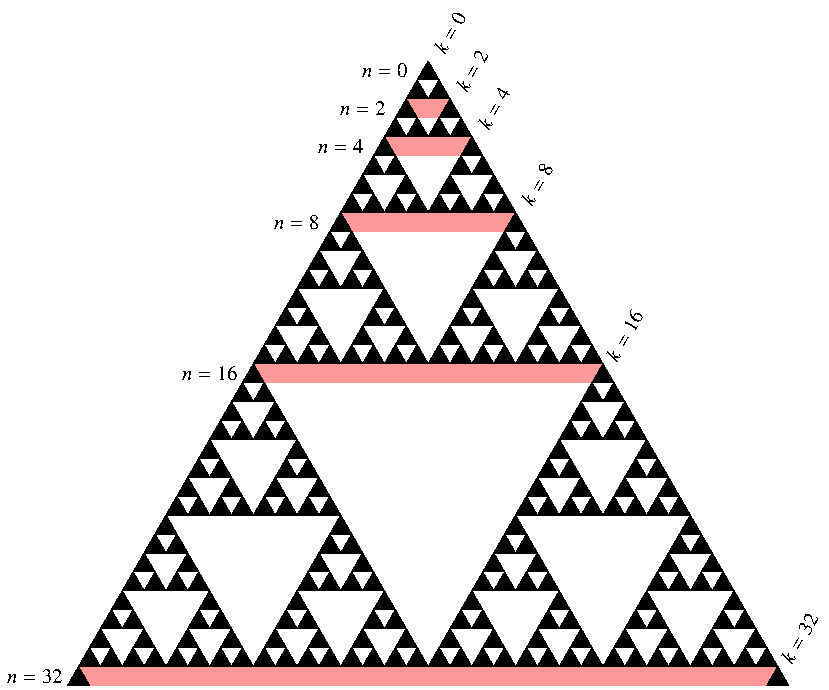
\includegraphics{chapters/30-endlichekoerper/images/binomial2.pdf}
\caption{Binomialkoeffizienten module $2$ im Pascal-Dreieck.
Auf den rot hinterlegten Zeilen, die zu Exponenten der Form $2^k$ gehören,
sind alle Koeffizienten ausser dem ersten und letzten durch $2$ teilbar.
\label{buch:endliche-koerper:fig:binomial2}}
\end{figure}
\bgroup
\definecolor{farbe1}{rgb}{0,0,0}
\definecolor{farbe2}{rgb}{1,0,0}
\definecolor{farbe3}{rgb}{0,0.6,0}
\definecolor{farbe4}{rgb}{0,0,1}

\begin{figure}
\centering
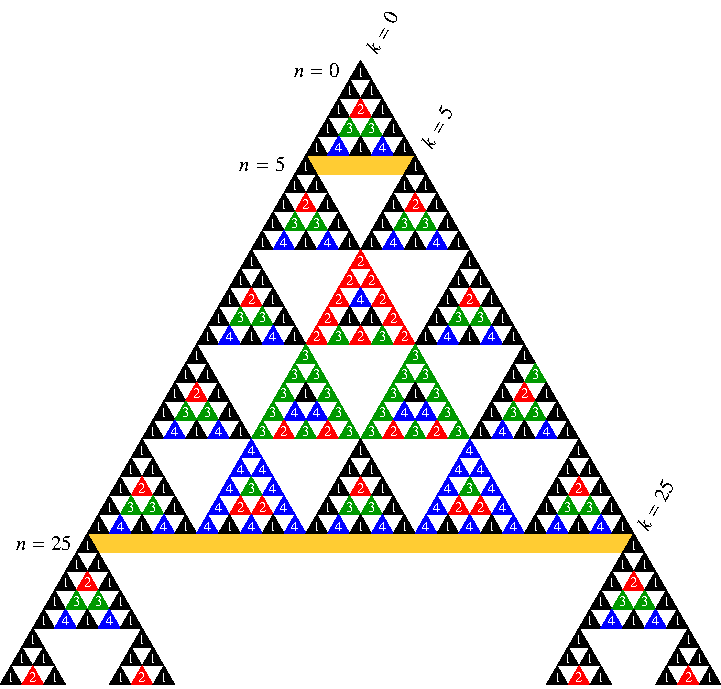
\includegraphics{chapters/30-endlichekoerper/images/binomial5.pdf}
\caption{Binomialkoeffizienten module $5$ im Pascal-Dreieck.
Die von $0$ verschiedenen Reste werden durch Farben dargestellt:
$1=\text{schwarz}$,
$2=\text{\color{farbe2}rot}$,
$3=\text{\color{farbe3}grün}$,
$4=\text{\color{farbe4}blau}$.
Auf den gelb hinterlegten Zeilen, die zu Exponenten der Form $5^k$ gehören,
sind alle Koeffizienten ausser dem ersten und letzten durch $5$ teilbar.
\label{buch:endliche-koerper:fig:binomial5}}
\end{figure}
\egroup
Die Abbildung~\ref{buch:endliche-koerper:fig:binomial2} zeigt den
Rest bei Teilung durch $2$ der Binomialkoeffizienten.
Man kann daraus ablesen, dass $\binom{n}{m}\equiv 0\mod 2$ für $n=2^k$ 
und $0<m<n$.
Abbildung~\ref{buch:endliche-koerper:fig:binomial5} zeigt das Pascal-Dreieck
auch noch für $p=5$.
Hier ist auch schön die Selbstähnlichkeit des Pascal-Dreiecks erkennbar.
Ersetzt man die ``5er-Dreiecke'' durch ein volles Dreieck mit der Farbe
des kleinen Dreiecks an seiner Spitze, entsteht wieder das ursprüngliche
Pascal-Dreieck.
Dabei gehen die Zeilen aus lauter Nullen ausser an den Enden ineinander über.

\begin{satz}
\label{buch:endliche-koerper:satz:binom}
Sei $p$ eine Primzahl, dann ist
\[
\binom{p}{m} \equiv 0\mod p
\]
für $0<m<n$.
\end{satz}

\begin{proof}[Beweis]
Für den Binomialkoeffizienten gilt
\[
\binom{p}{m}
=
\frac{p\cdot (p-1)\cdot(p-2)\cdot\ldots\cdot (p-m+1)}{1\cdot 2\cdot 3\cdot\ldots\cdot m}.
\]
Für $m<p$ kann keiner der Faktoren im Nenner $p$ sein, der Faktor $p$
im Zähler kann also nicht weggekürzt werden, so dass der Binomialkoeffizient
durch $p$ teilbar sein muss.
\end{proof}

\begin{satz}
\label{buch:endliche-koerper:satz:binomk}
Sei $p$ eine Primzahl, dann ist
\begin{equation}
\binom{p^k}{m} \equiv 0\mod p
\label{buch:endliche-koerper:eqn:a+b^p^k}
\end{equation}
für $0<m<p^k$
\end{satz}

\begin{proof}[Beweis]
Wir wissen aus Satz \ref{buch:endliche-koerper:satz:binom}, dass 
\begin{equation}
(a+b)^p = a^p+b^p.
\label{buch:endliche-koerper:eqn:a+b^p}
\end{equation}
Wir müssen zeigen, dass $(a+b)^{p^k}=a^{p^k}+b^{p^k}$ gilt.
Wir verwenden vollständige Induktion, 
\eqref{buch:endliche-koerper:eqn:a+b^p} ist die Induktionsverankerung.
Wir nehmen jetzt im Sinne der Induktionsannahme an, dass
\eqref{buch:endliche-koerper:eqn:a+b^p^k} für ein bestimmtes $k$ gilt.
Dann ist
\[
(a+b)^{p^{k+1}}
=
(a+b)^{p^k\cdot p}
=
\bigl((a+b)^{p^k}\bigr)^p
=
(a^{p^k}+b^{p^k})^p
=
a^{p^k\cdot p}+b^{p^k\cdot p}
=
a^{p^{k+1}}
+
b^{p^{k+1}},
\]
also die Behauptung für $k+1$.
Damit ist
\eqref{buch:endliche-koerper:eqn:a+b^p^k} für alle $k$ bewiesen.
\end{proof}

Die Aussage von Satz~\ref{buch:endliche-koerper:satz:binomk} kann man 
auch im Körper $\mathbb{F}_p$ formulieren:

\begin{satz}
\label{buch:endliche-koerper:satz:binomFp}
In $\mathbb{F}_p$ gilt
\[
\binom{p^k}{m}=0
\]
für beliebige $k>0$ und $0<m<p^k$.
\end{satz}

\subsubsection{Frobenius-Automorphismus}
Die Abbildung $x\mapsto x^n$ ist weit davon entfernt, sich mit den
algebraischen Strukturen zu vertragen.
Zum Beispiel kann man nicht erwarten, dass $(a+b)^n = a^n + b^n$,
denn nach der binomischen Formel
\begin{equation}
(a+b)^n
=
\sum_{k=0}^n \binom{n}{k} a^k b^{n-k}
=
a^n + \binom{n}{1}a^{n-1}b + \dots + \binom{n}{n-1}ab^{n-1} + b^n
\label{buch:endliche-koerper:fig:binomischeformel}
\end{equation}
gibt es zwischen den Termen an den Enden des Ausdrucks noch viele
Zwischenterme, die normalerweise nicht verschwinden.

Ganz anders sieht die Situation aus, wenn $n=p$ ist.
Nach Satz~\ref{buch:endliche-koerper:satz:binomFp} verschwinden die
Binomialkoeffizienten der Zwischenterme der Summe
\eqref{buch:endliche-koerper:fig:binomischeformel}
als Elemente von $\mathbb{F}_p$.
Daher gilt

\begin{satz}[Frobenius-Automorphismus]
In einem Körper $\Bbbk$ der Charakteristik $p$ ist die Abbildung
$x\mapsto x^p$ ist ein Automorphismus, der den Primkörper 
$\mathbb{F}_p\subset\Bbbk$ fest lässt.
\end{satz}

\begin{proof}[Beweis]
Wir müssen uns nur noch davon überzeugen, dass $\mathbb{F}_p\subset\Bbbk$
fest bleibt.
Nach dem kleine Satz von Fermat~\ref{buch:endliche-koerper:satz:fermat}
ist $a^p=a$ für alle $a\in\mathbb{F}_p$, der Frobenius-Automorphismus
lässt also alle Elemente von $\mathbb{F}_p$ fest.
\end{proof}

\begin{definition}
Der Automorphismus $x\mapsto x^p$ heisst {\em Frobenius-Automorphismus}.
\end{definition}

%
% wurzeln.tex -- Wurzeln einem endlichen Körper hinzufügen
%
% (c) 2021 Prof Dr Andreas Müller, Hochschule Rapperswil
%
% !TeX spellcheck = de_CH
\section{Wurzeln
\label{buch:section:wurzeln}}
\rhead{Wurzeln}
Im Körper $\mathbb{Q}$ kann man zum Beispiel die Wurzel aus $2$ nicht 
ziehen.
Das Problem haben wir in Abschnitt~\ref{buch:section:reelle-zahlen}
dadurch gelöst, dass wir $\mathbb{Q}$ zu den reellen Zahlen $\mathbb{R}$
erweitert haben.
Es ist aber auch möglich, nur die Zahl $\sqrt{2}$ hinzuzufügen,
so entsteht der Körper $\mathbb{Q}(\sqrt{2})$.
Das Problem dabei ist, was denn eigentlich $\sqrt{2}$ überhaupt ist.
Solange man die reellen Zahlen nicht hat, hat man auch $\sqrt{2}$ nicht.
Das Problem wird akut bei den endlichen Körpern wie zum Beispiel
$\mathbb{F}_3$,
da man diese nicht in $\mathbb{R}$ einbetten kann, also keine
bekannte Menge von Zahlen existiert, in der wir die Wurzel $\sqrt{2}$
finden könnte.

Im Altertum fiel dieses Problem zunächst den Pythagoreern auf.
Wenn $\sqrt{2}$ kein Bruch ist, was ist es dann?
Im 15.~Jahrhundert stellte sich dieses Problem bei den Versuchen, die
kubische Gleichung allgemein zu lösen, erneut.
Hier war es die Wurzel $\sqrt{-1}$, die den reellen Zahlen hinzuzufügen
war.
In $\mathbb{R}$ hat $\sqrt{-1}$ sicher keinen Platz, also wo existert
es denn überhaupt?
Auch der von Descartes eingeführte, eher unglückliche Begriff
``imaginäre Zahl'' illustriert dieses Dilemma.

Inzwischen hat man sich daran gewöhnt, dass man einfach ein neues Symbol
wählt, die algebraischen Regeln postuliert, nach denen damit zu rechnen
ist, und dann hofft oder besser beweist, dass keine Widersprüche auftreten.
Auf diese Weise kann man einem Körper $\Bbbk$ eine beliebige 
Nullstelle $\alpha$ eines Polynoms $f\in\Bbbk[X]$ mit Koeffizienten
in $\Bbbk$ hinzufügen und so den Körper $\Bbbk(\alpha)$ konstruieren.
Trotzdem bleibt die Frage offen: was {\em ist} denn eigentlich $\alpha$?

In diesem Abschnitt werden Wurzeln wie folgt konstruiert.
Zunächst wird in Abschnitt~\ref{buch:subsection:koerpererweiterungen}
gezeigt, dass man immer eine Matrix $M_\alpha$ finden kann, welche
genau die algebraischen Eigenschaften einer Nullstelle $\alpha$ eines
Polynoms hat.
Die Frage ``Was ist $\alpha$?'' erhält also die Antwort ``Eine Matrix''.
Mit diesem Bild lassen sich alle Körperoperationen realisieren, die
Inverse kann zum Beispiel als die inverse Matrix mit dem
Gauss-Algorithmus berechnet werden.
In einem zweiten Schritt zeigen wir dann, dass man die Rechnung noch
etwas vereinfachen kann, wenn man in Polynomringen arbeitet.
Schliesslich zeigen wir dann im
Abschnitt~\ref{buch:subsection:zerfaellungskoerper}, wie man 
den Prozess iterieren kann und so für beliebige Polynome immer einen
Körper finden kann, der alle Nullstellen enthält.
Wir beginnen in Abschnitt~\ref{buch:subsection:irreduziblepolynome}
damit, die Polynome, die für die Konstruktion in Frage kommen, etwas
genauer zu charakterisieren.

\subsection{Irreduzible Polynome
\label{buch:subsection:irreduziblepolynome}}
Die Zahlen, die man dem Körper hinzufügen möchte, müssen Nullstellen
eines Polynoms sein.
Wir gehen daher davon aus, dass $f\in \Bbbk[X]$ ein Polynom mit
Koeffizienten in $\Bbbk$ ist, dessen Nullstelle $\alpha$ hinzugefügt
werden sollen.
Das Ziel ist natürlich, dass diese Erweiterung vollständig beschrieben
werden kann durch das Polynom, ganz ohne Bezug zum Beispiel auf einen
numerischen Wert der Nullstelle, der ohnehin nur in $\mathbb{C}$ sinnvoll
wäre.

Nehmen wir jetzt an, dass sich das Polynom $f$ faktorisieren lässt.
Dann gibt es Polynome $g,h\in\Bbbk[X]$ derart, dass $f=g\cdot h$.
Die Polynome $g$ und $h$ haben geringeren Grad als $f$. 
Setzt man die Nullstelle $\alpha$ ein, erhält man
$0=f(\alpha)=g(\alpha)h(\alpha)$, daher muss einer der Faktoren
verschwinden, also $g(\alpha)=0$ oder $h(\alpha)=0$.
Ohne Beschränkung der Allgemeinheit kann angenommen werden, dass
$g(\alpha)=0$.
Die Operation des Hinzufügens der Nullstelle $\alpha$ von $f$
muss also genauso gut mit $g$ ausgeführt werden können.
Indem wir diese Überlegung auf $g$ anwenden können wir schliessen,
dass es ein Polynom $m\in\Bbbk[X]$ kleinstmöglichen Grades geben muss,
welches $\alpha$ als Nullstelle hat.
Zusätzlich kann verlangt werden, dass das Polynom normiert ist.

\begin{definition}
Ein Polynom $f\in \Bbbk[X]$ heisst {\em irreduzibel}, wenn es sich nicht
in zwei Faktoren $g,h\in \Bbbk[X]$ mit $f=gh$ zerlegen lässt.
\index{irreduzibles Polynom}%
\end{definition}

Für die Konstruktion des Körpers $\Bbbk(\alpha)$ muss daher ein irreduzibles
Polynom verwendet werden.

\begin{beispiel}
Das Polynom $f(X)=X^2-2$ ist in $\mathbb{Q}[X]$, es hat die beiden
Nullstellen $\sqrt{2}$ und $-\sqrt{2}$.
Beide Nullstellen haben die exakt gleichen algebraischen Eigenschaften,
sie sind mit algebraischen Mitteln nicht zu unterscheiden.
Nur die Vergleichsrelation ermöglicht, die negative Wurzel von der
positiven zu unterscheiden.
Das Polynom kann in $\mathbb{Q}$ nicht faktorisiert werden, denn die
einzig denkbare Faktorisierung ist $(X-\sqrt{2})(X+\sqrt{2})$, die
Faktoren sind aber keine Polynome in $\mathbb{Q}[X]$.
Also ist $f(X) = X^2 - 2$ ein irreduzibles Polynom über $\mathbb Q$.

Man kann das Polynom aber auch als Polynom in $\mathbb{F}_{23}[X]$
betrachten.
Im Körper $\mathbb{F}_{23}$ kann man durch probieren zwei Nullstellen
finden:
\begin{align*}
5^2 &= 25\equiv 2\mod 23
\\
\text{und}\quad
18^2 &=324 \equiv 2 \mod 23.
\end{align*}
Und tatsächlich ist in $\mathbb{F}_{23}[X]$
\[
(X-5)(X-18) = X^2 -23X+90
\equiv
X^2 -2 \mod 23,
\]
über $\mathbb{F}_{23}$ ist das Polynom $X^2-2$ also reduzibel.
\end{beispiel}

\begin{beispiel}
Die Zahl 
\[
\alpha = \frac{1+i\sqrt{3}}2
\]
ist eine Nullstelle des Polynoms $f(X)=X^3-1\in\mathbb{Z}[X]$.
$\alpha$ enthält aber nur Quadratwurzeln, man würde also eigentlich
erwarten, dass $\alpha$ Nullstelle eines quadratischen Polynoms ist.
Tatsächlich ist $f(X)$ nicht irreduzibel,  es ist nämlich
\[
X^3-1 = (X-1)(X^2+X+1).
\]
Da $\alpha$ nicht Nullstelle des ersten Faktors ist, muss es Nullstelle
des Polynoms $m(X)=X^2+X+1$ sein.
Der zweite Faktor ist irreduzibel.

Das Polynom $m(X)$ kann man aber auch als Polynom in $\mathbb{F}_7$ 
ansehen.
Dann kann man aber zwei Nullstellen finden,
\[
\begin{aligned}
X&=2&&\Rightarrow& 2^2+2+1=4+2+1&\equiv 0\mod 7
\\
X&=4&&\Rightarrow& 4^2+4+1=16+4+1=21&\equiv 0\mod 7.
\end{aligned}
\]
Dies führt auf die Faktorisierung
\[
(X-2)(X-4)
\equiv
(X+5)(X+3)
=
X^2+8X+15
\equiv
X^2+X+1\mod 7.
\]
Das Polynom $X^2+X+1$ ist daher über $\mathbb{F}_7$ reduzibel und
das Polynom $X^3-1\in\mathbb{F}_7$ zerfällt daher in Linearfaktoren
$X^3-1=(X+6)(X+3)(X+5)$.
\end{beispiel}


\subsection{Körpererweiterungen
\label{buch:subsection:koerpererweiterungen}}
Nach den Vorbereitungen von
Abschnitt~\ref{buch:subsection:irreduziblepolynome}
können wir jetzt definieren, wie die Körpererweiterung
konstruiert werden soll.

\subsubsection{Erweiterung mit einem irreduziblen Polynom}
Sei $m\in\Bbbk[X]$ ein irreduzibles Polynome über $\Bbbk$ mit dem Grad
$\deg m=n$,
wir dürfen es als normiert annehmen und schreiben es in der Form
\[
m(X)
=
m_0+m_1X+m_2X^2 + \dots m_{n-1}X^{n-1}+X^n.
\]
Wir möchten den Körper $\Bbbk$ um eine Nullstelle $\alpha$ von $m$
erweitern.
Da es in $\Bbbk$ keine Nullstelle von $m$ gibt, konstruieren wir
$\Bbbk(\alpha)$ auf abstrakte Weise, ganz so wie das mit der imaginären
Einheit $i$ gemacht wurde.
Die Zahl $\alpha$ ist damit einfach ein neues Symbol, mit dem man
wie in der Algebra üblich rechnen kann.
Die einzige zusätzliche Eigenschaft, die von $\alpha$ verlangt wird,
ist dass $m(\alpha)=0$.
Unter diesen Bedingungen können beliebige Ausdrücke der Form
\begin{equation}
a_0 + a_1\alpha + a_2\alpha^2 + \dots a_k\alpha^k
\label{buch:endlichekoerper:eqn:ausdruecke}
\end{equation}
gebildet werden.
Aus der Bedingung $m(\alpha)=0$ folgt aber, dass
\begin{equation}
\alpha^n = -m_{n-1}\alpha^{n-1} -\dots - m_2\alpha^2  - m_1\alpha - m_0.
\label{buch:endlichekoerper:eqn:reduktion}
\end{equation}
Alle Potenzen mit Exponenten $\ge n$ in
\eqref{buch:endlichekoerper:eqn:ausdruecke}
können daher durch die rechte Seite von
\eqref{buch:endlichekoerper:eqn:reduktion}
ersetzt werden.
Als Menge ist daher
\[
\Bbbk(\alpha)
=
\{
a_0+a_1\alpha+a_2\alpha^2+\dots+a_{n-1}\alpha^{n-1}\;|\; a_i\in\Bbbk\}
\]
ausreichend.
Die Addition von solchen Ausdrücken und die Multiplikation mit Skalaren
aus $\Bbbk$ machen $\Bbbk(\alpha)\cong \Bbbk^n$ zu einem Vektorraum,
die Operationen können auf den Koeffizienten komponentenweise ausgeführt
werden.

\subsubsection{Matrixrealisierung der Multiplikation mit $\alpha$}
Die schwierige Operation ist die Multiplikation mit $\alpha$.
Dazu stellen wir zusammen, wie die Multiplikation mit $\alpha$ auf den
Basisvektoren von $\Bbbk(\alpha)$ wirkt:
\[
\alpha\colon
\Bbbk^n\to\Bbbk^n
:
\left\{
\begin{aligned}
     1  &\mapsto \alpha   \\
\alpha  &\mapsto \alpha^2 \\
\alpha^2&\mapsto \alpha^3 \\
        &\phantom{m}\vdots\\
\alpha^{n-2}&\mapsto \alpha^{n-1}\\
\alpha^{n-1}&\mapsto \alpha^n = -m_0-m_1\alpha-m_2\alpha^2-\dots-m_{n-1}\alpha^{n-1}
\end{aligned}
\right.
\]
Diese lineare Abbildung hat die Matrix
\[
M_{\alpha}
=
\begin{pmatrix}
0   &    &    &      &   &-m_0    \\
1   & 0  &    &      &   &-m_1    \\
    & 1  & 0  &      &   &-m_2    \\
    &    & 1  &\ddots&   &\vdots  \\
    &    &    &\ddots& 0 &-m_{n-2}\\
    &    &    &      & 1 &-m_{n-1}
\end{pmatrix}.
\]
%TODO: Was ist hier die Aussage?
Aufgrund der Konstruktion die Lineare Abbildung $m(M_\alpha)$,
die man erhält, wenn
man die Matrix $M_\alpha$ in das Polynom $m$ einsetzt, jeden Vektor
in $\Bbbk(\alpha)$ zu Null machen.
Als Matrix muss daher $m(M_\alpha)=0$ sein.
Dies kann man auch mit einem Computeralgebra-System nachprüfen.

\begin{beispiel}
In einem früheren Beispiel haben wir gesehen, dass
$\alpha=\frac12(-1+\sqrt{3})$ 
eine Nullstelle des irreduziblen Polynomes $m(X)=X^2+X+1$ ist.
Die zugehörige Matrix $M_\alpha$ ist
\[
M_{\alpha}
=
\begin{pmatrix}
0&-1\\
1&-1
\end{pmatrix}
\qquad\Rightarrow\qquad
M_{\alpha}^2
=
\begin{pmatrix}
-1& 1\\
-1& 0
\end{pmatrix},\quad
M_{\alpha}^3
=
\begin{pmatrix}
 1& 0\\
 0& 1
\end{pmatrix}.
\]
Wir können auch verifizieren, dass
\[
m(M_\alpha)
=
M_\alpha^2+M_\alpha+I
=
\begin{pmatrix}
-1& 1\\
-1& 0
\end{pmatrix}
+
\begin{pmatrix}
0&-1\\
1&-1
\end{pmatrix}
+
\begin{pmatrix}
1&0\\
0&1
\end{pmatrix}
=
\begin{pmatrix}
0&0\\
0&0
\end{pmatrix}.
\]
Die Matrix ist also eine mögliche Realisierung für das ``mysteriöse''
Element $\alpha$.
Es hat alle algebraischen Eigenschaften von $\alpha$.
\end{beispiel}

Die Menge $\Bbbk(\alpha)$ kann durch die Abbildung $\alpha\mapsto M_\alpha$
mit der Menge aller Matrizen
\[
\Bbbk(M_\alpha)
=
\left\{
\left.
a_0I+a_1M_\alpha+a_2M_\alpha^2+\dots+a_{n-1}M_\alpha^{n-1}\;\right|\; a_i\in\Bbbk
\right\}
\]
in eine Eins-zu-eins-Beziehung gebracht werden.
Diese Abbildung ist ein Algebrahomomorphismus.
Die Menge $\Bbbk(M_\alpha)$ ist also das Bild des
Körpers $\Bbbk(\alpha)$ in der Matrizenalgebra $M_n(\Bbbk)$.

\subsubsection{Inverse}
Im Moment wissen wir noch nicht, wie wir $\alpha^{-1}$ berechnen sollten.
Wir können aber auch die Matrizendarstellung verwenden.
Für Matrizen wissen wir selbstverständlich, wie Matrizen invertiert
werden können.
Tatsächlich kann man die Matrix $M_\alpha$ direkt invertieren:
\[
M_\alpha^{-1}
=
\frac{1}{m_0}
\begin{pmatrix}
   -m_1 &m_0&   &      &      &   \\
   -m_2 & 0 &m_0&      &      &   \\
   -m_3 &   & 0 &   m_0&      &   \\
 \vdots &   &   &\ddots&\ddots&   \\
-m_{n-1}& 0 & 0 &      &  0   &m_0\\
    -1  & 0 & 0 &      &  0   & 0
\end{pmatrix},
\]
wie man durch Ausmultiplizieren überprüfen kann:
\[
\frac{1}{m_0}
\begin{pmatrix}
   -m_1 &m_0&   &      &      &   \\
   -m_2 & 0 &m_0&      &      &   \\
   -m_3 &   & 0 &   m_0&      &   \\
 \vdots &   &   &\ddots&\ddots&   \\
-m_{n-1}& 0 & 0 &      &  0   &m_0\\
    -1  & 0 & 0 &      &  0   & 0
\end{pmatrix}
\begin{pmatrix}
  0   &    &    &      &   &-m_0    \\
  1   & 0  &    &      &   &-m_1    \\
      & 1  & 0  &      &   &-m_2    \\
      &    & 1  &\ddots&   &\vdots  \\
      &    &    &\ddots& 0 &-m_{n-2}\\
      &    &    &      & 1 &-m_{n-1}
\end{pmatrix}
=
\begin{pmatrix}
1&0&0&\dots&0&0\\
0&1&0&\dots&0&0\\
0&0&1&\dots&0&0\\
\vdots&\vdots&\vdots&\ddots&\vdots\\
0&0&0&\dots&1&0\\
0&0&0&\dots&0&1
\end{pmatrix}
\]
Die Invertierung in $\Bbbk(M_\alpha)$ ist damit zwar geklärt, aber
es wäre viel einfacher, wenn man die Inverse auch in $\Bbbk(\alpha)$
bestimmen könnte.

Die Potenzen von $M_\alpha^k$ haben in der ersten Spalte genau in
Zeile $k+1$ eine $1$, alle anderen Einträge in der ersten Spalte
sind $0$.
Die erste Spalte eines Elementes
$a(\alpha)=a_0+a_1\alpha+a_2\alpha^2 +a_{n-1}\alpha^{n-1}$
besteht daher genau aus den Elementen $a_i$.
Die Inverse des Elements $a$ kann daher wie folgt gefunden werden.
Zunächst wird die Matrix $a(M_\alpha)$ gebildet und invertiert.
Wir schreiben $B=a(M_\alpha)^{-1}$.
Aus den Einträgen der ersten Spalte kann man jetzt die Koeffizienten
\[
b_0=(B)_{11},
b_1=(B)_{21},
b_2=(B)_{31},\dots,
b_{n-1}=(B)_{n,1}
\]
ablesen und daraus das Element
\[
b(\alpha) = b_0+b_1\alpha+b_2\alpha^2 + \dots + b_{n-1}\alpha^{n-1}
\]
bilden.
Da $b(M_\alpha)=B$ die inverse Matrix von $a(M_\alpha)$ ist, muss $b(\alpha)$
das Inverse von $a(\alpha)$ sein.

\begin{beispiel}
Wir betrachten das Polynom 
\[
m(X) = X^3 + 2X^2 + 2X + 3 \in \mathbb{F}_{7}[X],
\]
es ist irreduzibel.
Sei $\alpha$ eine Nullstelle von $m$, wir suchen das inverse Element zu
\[
a(\alpha)=1+2\alpha+2\alpha^2\in\mathbb{F}_{7}(\alpha).
\]
Die Matrix $a(M_\alpha)$ bekommt die Form
\[
A=\begin{pmatrix}
 1& 1& 6\\
 2& 4& 5\\
 2& 5& 1
\end{pmatrix}.
\]
Die Inverse kann man bestimmen, indem man den
Gauss-Algorithmus in $\mathbb{F}_{7}$ durchführt.
Die Arithmetik in $\mathbb{F}_{7}$ ist etwas ungewohnt, insbesondere
die Pivot-Division ist etwas mühsam, daher sind in
Abbildung~\ref{buch:endlichekoerper:fig:additionmultiplikation}
die Additions- und Multiplikationstabellen zusammengestellt.
\begin{figure}
\begin{center}
\begin{tabular}{|>{$}c<{$}|>{$}c<{$}>{$}c<{$}>{$}c<{$}>{$}c<{$}>{$}c<{$}>{$}c<{$}>{$}c<{$}|}
\hline
+&0&1&2&3&4&5&6\\
\hline
0&0&1&2&3&4&5&6\\
1&1&2&3&4&5&6&0\\
2&2&3&4&5&6&0&1\\
3&3&4&5&6&0&1&2\\
4&4&5&6&0&1&2&3\\
5&5&6&0&1&2&3&4\\
6&6&0&1&2&3&4&5\\
\hline
\end{tabular}
\qquad
\begin{tabular}{|>{$}c<{$}|>{$}c<{$}>{$}c<{$}>{$}c<{$}>{$}c<{$}>{$}c<{$}>{$}c<{$}>{$}c<{$}|}
\hline
\cdot
 &0&1&2&3&4&5&6\\
\hline
0&0&0&0&0&0&0&0\\
1&0&1&2&3&4&5&6\\
2&0&2&4&6&1&3&5\\
3&0&3&6&2&5&1&4\\
4&0&4&1&5&2&6&3\\
5&0&5&3&1&6&4&2\\
6&0&6&5&4&3&2&1\\
\hline
\end{tabular}
\end{center}
\caption{Additions- und Multiplikationstabelle für das Rechnen im
Galois-Körper $\mathbb{F}_7$.
Die multiplikative Inverse eines Elements in $a\in\mathbb{F}_7^*$
findet man, indem man in der Multiplikationstabelle in der Zeile
$a$ die Spalte mit der $1$ sucht, diese Spalte ist mit der multiplikativen
Inversen von $a$ angeschrieben.
\label{buch:endlichekoerper:fig:additionmultiplikation}}
\end{figure}
Mit dieser Rechenhilfe kann jetzt der Gaussalgorithmus leicht durchgeführt
werden:
\begin{align*}
\begin{tabular}{|>{$}c<{$}>{$}c<{$}>{$}c<{$}|>{$}c<{$}>{$}c<{$}>{$}c<{$}|}
\hline
 1& 1& 6& 1& 0& 0\\
 2& 4& 5& 0& 1& 0\\
 2& 5& 1& 0& 0& 1\\
\hline
\end{tabular}
&\rightarrow
\begin{tabular}{|>{$}c<{$}>{$}c<{$}>{$}c<{$}|>{$}c<{$}>{$}c<{$}>{$}c<{$}|}
\hline
 1& 1& 6& 1& 0& 0\\
 0& 2& 0& 5& 1& 0\\
 0& 3& 3& 5& 0& 1\\
\hline
\end{tabular}
\rightarrow
\begin{tabular}{|>{$}c<{$}>{$}c<{$}>{$}c<{$}|>{$}c<{$}>{$}c<{$}>{$}c<{$}|}
\hline
 1& 1& 6& 1& 0& 0\\
 0& 1& 0& 6& 4& 0\\
 0& 0& 3& 1& 2& 1\\
\hline
\end{tabular}
\\
&\rightarrow
\begin{tabular}{|>{$}c<{$}>{$}c<{$}>{$}c<{$}|>{$}c<{$}>{$}c<{$}>{$}c<{$}|}
\hline
 1& 1& 6& 1& 0& 0\\
 0& 1& 0& 6& 4& 0\\
 0& 0& 1& 5& 3& 5\\
\hline
\end{tabular}
\\
&\rightarrow
\begin{tabular}{|>{$}c<{$}>{$}c<{$}>{$}c<{$}|>{$}c<{$}>{$}c<{$}>{$}c<{$}|}
\hline
 1& 1& 0& 6& 3& 5\\
 0& 1& 0& 6& 4& 0\\
 0& 0& 1& 5& 3& 5\\
\hline
\end{tabular}
\rightarrow
\begin{tabular}{|>{$}c<{$}>{$}c<{$}>{$}c<{$}|>{$}c<{$}>{$}c<{$}>{$}c<{$}|}
\hline
 1& 0& 0& 0& 6& 5\\
 0& 1& 0& 6& 4& 0\\
 0& 0& 1& 5& 3& 5\\
\hline
\end{tabular}
\end{align*}
Für die Durchführung braucht man die Inversen in $\mathbb{F}_7$
der Pivot-Elemente, sie sind $2^{-1}=4$ und $3^{-1}=5$.
Im rechten Teil des Tableau steht jetzt die inverse Matrix
\[
A^{-1}
=
B=\begin{pmatrix}
 0& 6& 5\\
 6& 4& 0\\
 5& 3& 5
\end{pmatrix}.
\]
Daraus können wir jetzt das inverse Element
\[
b(\alpha) = 6\alpha+5\alpha^2
\]
ablesen.
Das Produkt $b(X)\cdot a(X)$ ist
\begin{align*}
(1+2X+2X^2)(6X+5X^2)
&=
10X^4 + 22X^3 + 17X^2 + 6X
\\
&=
3X^4+X^3+3X^2+6X
\intertext{
Diese Polynom muss jetzt mit dem Minimalpolynom $m(X)$ reduziert
werden, wir subtrahieren dazu $3Xm(X)$ und erhalten}
&=
-5X^3-3X^2-3X
\\
&=
2X^3+4X^2+4X
\intertext{Die vollständige Reduktion wird erreicht, indem wir nochmals
$2m(X)$ subtrahieren:}
&=
-6 \equiv 1\mod 7,
\end{align*}
das Element $b(\alpha)=6\alpha+5\alpha^2$ ist also das Inverse Element von
$a(\alpha)=1+2\alpha+2\alpha^2$ in $\mathbb{F}_7(\alpha)$.
\label{buch:endlichekoerper:beispiel:inversemitmatrix}
\end{beispiel}

Die Matrixrealisation von $\Bbbk(\alpha)$ führt also auf eine effiziente
Berechnungsmöglichkeit für das Inverse eines Elements von $\Bbbk(\alpha)$.

\subsubsection{Algebraische Konstruktion}
Die Matrixdarstellung von $\alpha$ ermöglicht eine rein algebraische
und für die Rechnung besser geeignete Konstruktion.
Für jedes Polynom $f\in\Bbbk[X]$ ist $f(M_\alpha)\in M_n(\Bbbk)$.
Dies definiert einen Homomorphismus
\[
\varphi\colon \Bbbk[X] \to M_n(\Bbbk) : f \mapsto f(M_\alpha).
\]
Wir haben früher schon gesehen, dass das Bild dieses Homomorphismus
genau die Menge $\Bbbk(M_\alpha)$ ist.
Allerdings ist $\varphi$ nicht injektiv, das Polynom $m$ wird zum
Beispiel auf $\varphi(m) = m(M_\alpha) = 0$ abgebildet.

Der Kern von $\varphi$ besteht aus allen Polynomen $p\in\Bbbk[X]$,
für die $p(M_\alpha)=0$ gilt.
Da aber alle Matrizen $E,M_\alpha,\dots,M_\alpha^{n-1}$ linear
unabhängig sind, muss ein solches Polynom den gleichen Grad haben
we $m$, und damit ein Vielfaches von $m$ sein.
Der Kern besteht daher genau aus den Vielfachen von $m(X)$,
$\ker\varphi = m(X)\Bbbk[X]$.

Es ist nicht a priori klar, dass der Quotient $R/I$ für ein
Ideal $I\subset R$ ein Körper ist.
Hier spielt es eine Rolle, dass das von $m$ erzeugte Ideal
maximal ist im folgenden Sinne.

\begin{definition}
Ein Ideal $I\subset R$ heisst {\em maximal}, wenn für jedes andere Ideal
$J$ mit $I\subset J\subset R$ entweder $I=J$ oder $J=R$ gilt.
\end{definition}

\begin{beispiel}
Die Ideale $p\mathbb{Z}\subset \mathbb{Z}$ sind maximal genau dann, wenn
$p$ eine Primzahl ist.

TODO: XXX Begründung
\end{beispiel}

\begin{satz}
Der Ring $R/I$ ist genau dann ein Körper, wenn $I$ ein maximales Ideal ist.
\end{satz}

\begin{proof}[Beweis]
\end{proof}

Ein irreduzibles Polynom $m\in\Bbbk[X]$ erzeugt ein maximales Ideal,
somit ist $\Bbbk[X]/m\Bbbk[X]\cong \Bbbk(M_\alpha) \cong \Bbbk(\alpha)$.

\subsubsection{Reduktion modulo $m$}
Die algebraische Konstruktion hat gezeigt, dass die arithmetischen
Operationen im Körper $\Bbbk(\alpha)$ genau die Operationen 
in $\Bbbk[X]/m\Bbbk[X]$ sind.
Eine Zahl in $\Bbbk(\alpha)$ wird also durch ein Polynom vom 
$n-1$ dargestellt.
Addieren und Subtrahieren erfolgen Koeffizientenweise in $\Bbbk$.
Bei der Multiplikation entsteht möglicherwise ein Polynom grösseren
Grades, mit dem Polynomdivisionsalgorithmus kann der Rest bei Division
durch $m$ ermittelt werden.

\begin{beispiel}
Das Polyonom $f=X^5+X^4+X^3+X^2+X^1+1\in\mathbb{F}_7[X]$ soll modulo
$m(X)=X^3+2X^2+2X^2+3$ reduziert werden.
Wir führen die Polynomdivision in $\mathbb{F}_7[X]$ durch, die
Multiplikationstabelle von $\mathbb{F}_7$ in
Abbildung~\ref{buch:endlichekoerper:fig:additionmultiplikation}
ist dabei wieder hilfreich.
\[
\arraycolsep=1.4pt
\begin{array}{rcrcrcrcrcrcrcrcrcrcrcrcr}
X^5&+& X^4&+& X^3&+& X^2&+& X&+&1&:&X^3&+&2X^2&+&2X&+&3&=&X^2&+&6X&+&1\rlap{$\mathstrut=q$}\\
\llap{$-($}X^5&+&2X^4&+&2X^3&+&3X^2\rlap{$)$}& &  & & & &   & &    & &  & & & &   & &  & & \\
\cline{1-7}
   & &6X^4&+&6X^3&+&5X^2&+& X& & & &   & &    & &  & & & &   & &  & & \\
   & &\llap{$-($}6X^4&+&5X^3&+&5X^2&+&4X\rlap{$)$}& & & &   & &    & &  & & & &   & &  & & \\
\cline{3-9}
   & &    & & X^3& &    &+&4X&+&1& &   & &    & &  & & & &   & &  & & \\
   & &    & &\llap{$-($}X^3&+&2X^2&+&2X&+&3\rlap{$)$}& &   & &    & &  & & & &   & &  & & \\
\cline{5-11}
   & &    & &    & &5X^2&+&2X&+&5\rlap{$\mathstrut=r$}& &   & &    & &  & & & &   & &  & & \\
\end{array}
\]
Die Kontrolle
\[
\arraycolsep=1.4pt
\begin{array}{rcrcrcrcrcrcr}
\llap{$($}X^2&+&  6X&+&   1\rlap{$)$}&\cdot&\llap{$($} X^3&+&2X^2&+&2X&+&3\rlap{$)$}\\
\cline{1-13}
   & &    & &    &     & X^3&+&2X^2&+&2X&+&3\\
   & &    & &6X^4&  +  &5X^3&+&5X^2&+&4X& & \\
   & & X^5&+&2X^4&  +  &2X^3&+&3X^2& &  & & \\
\cline{3-13}
   & & X^5&+& X^4&  +  & X^3&+&3X^2&+&6X&+&3\rlap{$\phantom{)}=q\cdot m$}\\
   & &    & &    &     &    & &\llap{$+($}5X^2&+&2X&+&5\rlap{$)=r$}\\
\cline{3-13}
   & & X^5&+& X^4&  +  & X^3&+& X^2&+& X&+&1\\
\cline{3-13}
\end{array}
\]
zeigt $f=qm+r$ und damit die Korrektheit der Rechnung.
\end{beispiel}

Die Identität $m(\alpha)=0$ kann aber auch wie folgt interpretiert werden.
Sei der Grad von $f$ mindestens so gross wie der von $m$, also
$l=\deg f\ge \deg m=n$.
Indem man mit $\alpha^{l-n}$ multipliziert, erhält man die Relation
\[
\alpha^l + m_{n-1}\alpha^{l-1} + m_{n-2}\alpha^{l-2}+\dots +a_1\alpha^{l-n+1} + a_0\alpha^{l-n} = 0.
\]

Ist $f_l$ der führende Koeffizient des Polynoms $f$, dann ist
$f-f_0mX^{n-l}$ ein Polynom vom Grad $l-1$, welches modulo $m$
mit $f$ übereinstimmt.
Indem man dies wiederholt, kann man also die Reduktion finden, ohne
den Polynomdivisionsalgorithmus durchzuführen.
Man erhält auf diese Weise zwar den Quotienten $q$ nicht, aber den
Rest $r$ kann man trotzdem bekommen.

\begin{beispiel}
Wir wenden den eben beschriebenen Algorithmus wieder auf das
Polynom $f=X^5+X^4+X^3+X^2+X+1$ an und erhalten:
\[
\arraycolsep=1.4pt
\begin{array}{rcrcrcrcrcr}
X^5&+& X^4&+& X^3&+& X^2&+& X&+&1\\
\llap{$-($}X^5&+&2X^4&+&2X^3&+&3X^2\rlap{$\mathstrut =X^2m)$}& &  & & \\
\cline{1-11}
   & &6X^4&+&6X^3&+&5X^2&+& X&+&1\\
   & &\llap{$-($}6X^4&+&5X^3&+&5X^2&+&4X\rlap{$\mathstrut =6Xm)$}& & \\
\cline{3-11}
   & &    & & X^3& &    &+&4X&+&1\\
   & &    & & \llap{$-($}X^3&+&2X^2&+&2X&+&3\rlap{$\mathstrut =m)$}\\
\cline{5-11}
   & &    & &    & &5X^2&+&2X&+&5\rlap{$\mathstrut =r$}\\
\end{array}
\]
Dies ist derselbe Rest wie wir mit dem Divisionsalgorithmus
gefunden haben.
\end{beispiel}

Diese Form des Reduktionsalgorithmus ist besonders leicht durchzuführen
in einem Körper $\mathbb{F}_2$, da dort die Addition und die Subtraktion
der Koeffizienten übereinstimmen.
Die Multiplikation mit $X$ ist nichts anders als ein Shift der
Koeffizienten.

\subsubsection{Multiplikative Inverse}
Die schwierigste Operation in $\Bbbk(\alpha)$ ist die Division.
Wie bei der Berechnung der Inversion in einem Galois-Körper $\mathbb{F}_p$
kann dafür der euklidische Algorithmus verwendet werden.
Sei also $f\in\Bbbk[X]$ ein Polynom vom Grad $\deg f <\deg m$, es soll
das multiplikative Inverse gefunden werden.
Da $m$ ein irreduzibles Polynom ist, müssen $f$ und $m$ teilerfremd sein.
Der euklidische Algorithmus liefert zwei Polynome $s,t\in\Bbbk[X]$ derart,
dass
\[
sf+tm=1.
\]
Reduzieren wir modulo $m$, wird daraus $af=1$ in $\Bbbk[X]/m\Bbbk[X]$.
Das Polynom $a$, reduziert module $m$, ist also die multiplikative
Inverse von $f$.

Bei der praktischen Durchführung des euklidischen Algorithmus ist der 
letzte Rest $r_{n-1}$ oft nicht $1$ sondern ein anderes Element von
$\mathbb{F}_p^*$.
Die Linearkombination von $f$ und $m$ mit den berechneten Faktoren
$s$ und $t$ ist daher auch nicht $1$, sondern 
\[
sf+tm=r_{n-1}.
\]
Da aber alle Elemente in $\mathbb{F}_p^*$ invertierbar sind, kann man
durch $r_{n-1}$ dividieren, was
\[
r_{n-1}^{-1}sf+r_{n-1}^{-1}tm=1
\]
ergibt.
Also ist $r_{n-1}^{-1}s$ die gesuchte Inverse in $\mathbb{F}_p(\alpha)$,
dies passiert auch im folgenden Beispiel.

\begin{beispiel}
Auf 
Seite~\pageref{buch:endlichekoerper:beispiel:inversemitmatrix}
haben wir die multiplikative Inverse von
$f=2X^2+2X+1\in\mathbb{F}_7[X]/m\mathbb{F}_7[X]$ 
mit $m = X^3 + 2X^2 + 2X + 3$
mit Hilfe von Matrizen berechnet, hier soll sie jetzt nochmals
mit dem euklidischen Algorithmus berechnet werden.

Zunächst müssen wir den euklidischen Algorithmus für die beiden Polynome
$f$ und $m$ durchführen.
Der Quotient $m:f$ ist:
\[
\arraycolsep=1.4pt
\begin{array}{rcrcrcrcrcrcrcrcr}
  X^3&+&2X^2&+&2X&+&3&:&2X^2&+&2X&+&1&=&4X&+&4\rlap{$\mathstrut=q_0$}\\
\llap{$-($}X^3&+& X^2&+&4X\rlap{$)$}& & & &    & &  & & & &  & & \\ \cline{1-5}
     & & X^2&+&5X&+&3& &    & &  & & & &  & & \\
     &&\llap{$-(\phantom{2}$}X^2&+& X&+&4\rlap{$)$}& &    & &  & & & &  & & \\ \cline{3-7}
     & &    & &4X&+&6\rlap{$\mathstrut=r_0$}& &    & &  & & & &  & &
\end{array}
\]
Jetzt muss der Quotient $f:r_0$ berechnet werden:
\[
\arraycolsep=1.4pt
\begin{array}{rcrcrcrcrcrcrcrcr}
  2X^2&+&2X&+&1&:&4X&+&6&=&4X&+&5\rlap{$\mathstrut=q_1$}\\
\llap{$-($}2X^2&+&3X\rlap{$)$}& & & &  & & & &  \\ \cline{1-3}
      & &6X&+&1& &  & & & &  \\
      & &\llap{$-($}6X&+&2\rlap{$)$}& &  & & & &  \\ \cline{3-5}
      & &  & &6\rlap{$\mathstrut=r_1$}& & & &  & & & &
\end{array}
\]
Da der Rest $r_1\in\mathbb{F}_7^*$ liegt, gibt die nächste Division
natürlich den Rest $0$ und der letzte nicht verschwindende Rest ist
$r_{1}=6$:
\[
\arraycolsep=1.4pt
\begin{array}{rcrcrcrcr}
4X&+&6&:&6&=&3X&+&1\rlap{$\mathstrut=q_2$} \\
\llap{$-($}4X\rlap{$)$}& & & & & &  & &  \\ \cline{1-1}
 0&+&6& & & &  & & \\
  & &\llap{$-($}6\rlap{$)$}& & & &  & &\\ \cline{3-3}
  & &0\rlap{$\mathstrut=r_2$}& & & &  & &
\end{array}
\]
Damit ist der euklidische Algorithmus abgeschlossen.

Durch Ausmultiplizieren der Matrizen $Q(-q_i)$ können wir jetzt auch die 
Faktoren $s$ und $t$ finden.
\begin{align*}
Q=\begin{pmatrix}
s&t\\
*&*
\end{pmatrix}
&= Q(q_2)Q(q_1)Q(q_0)
=
\begin{pmatrix}0&1\\1&-q_2\end{pmatrix}
\begin{pmatrix}0&1\\1&-q_1\end{pmatrix}
\begin{pmatrix}0&1\\1&-q_0\end{pmatrix}
\\
&=
\begin{pmatrix}
0&1\\
1&4X+6
\end{pmatrix}
\begin{pmatrix}
0&1\\
1&3X+2
\end{pmatrix}
\begin{pmatrix}
0&1\\
1&3X+3
\end{pmatrix}
\\
&=
\begin{pmatrix}
0&1\\
1&4X+6
\end{pmatrix}
\begin{pmatrix}
   1&3X+3\\
3X+2&2X^2 + X
\end{pmatrix}
\\
&=
\begin{pmatrix}
3X+2           &2X^2+X\\
1+(4X+6)(3X+2) &3X+3 + (4X+6)(2X^2+X)
\end{pmatrix}
\\
&=
\begin{pmatrix}
     3X+2 & 2X^2     +X\\
5X^2+5X+6 &  X^3+2X^2+2X+6
\end{pmatrix}
\end{align*}
Daraus liest man
\[
s
=
2X^2+X
\qquad\text{und}\qquad
t
=
3X+2
\]
ab.
Wir überprüfen, ob die Koeffizienten der ersten Zeile tatsächlich $m$ und $f$
zu $r_1=6$ kombinieren.
Es ist
\begin{align*}
(3X+2)\cdot m + (2X^2+X)\cdot f
&= 
(3X+2)
(X^3+3X^2+X+2)
+
(2X^2+X)
(2X^2+2X+1)
=
6=r_1
\end{align*}
Die multiplikative Inverse ist daher
$
r_1^{-1}(2X^2 + X)
=
6^{-1}
(2X^2 + X)
=
6
(2X^2 + X)
=
5X^2+6X$,
was mit dem Beispiel von
Seite~\pageref{buch:endlichekoerper:beispiel:inversemitmatrix}
übereinstimmt.
\end{beispiel}

Besonders einfach ist die Rechung für $\Bbbk=\mathbb{F}_2$.
Dieser Spezialfall ist für die praktische Anwendung in der Kryptographie
von besonderer Bedeutung, daher wird er im 
In Kapitel~\ref{buch:chapter:kryptographie} genauer untersucht.

\subsection{Zerfällungskörper
\label{buch:subsection:zerfaellungskoerper}}
XXX TODO







\section*{Übungsaufgaben}
\rhead{Übungsaufgaben}
\aufgabetoplevel{chapters/30-endlichekoerper/uebungsaufgaben}
\begin{uebungsaufgaben}
\uebungsaufgabe{3004}
\uebungsaufgabe{3003}
\uebungsaufgabe{3002}
\uebungsaufgabe{3001}
\uebungsaufgabe{3005}
\end{uebungsaufgaben}

